\documentclass[1p]{elsarticle_modified}
%\bibliographystyle{elsarticle-num}

%\usepackage[colorlinks]{hyperref}
%\usepackage{abbrmath_seonhwa} %\Abb, \Ascr, \Acal ,\Abf, \Afrak
\usepackage{amsfonts}
\usepackage{amssymb}
\usepackage{amsmath}
\usepackage{amsthm}
\usepackage{scalefnt}
\usepackage{amsbsy}
\usepackage{kotex}
\usepackage{caption}
\usepackage{subfig}
\usepackage{color}
\usepackage{graphicx}
\usepackage{xcolor} %% white, black, red, green, blue, cyan, magenta, yellow
\usepackage{float}
\usepackage{setspace}
\usepackage{hyperref}

\usepackage{tikz}
\usetikzlibrary{arrows}

\usepackage{multirow}
\usepackage{array} % fixed length table
\usepackage{hhline}

%%%%%%%%%%%%%%%%%%%%%
\makeatletter
\renewcommand*\env@matrix[1][\arraystretch]{%
	\edef\arraystretch{#1}%
	\hskip -\arraycolsep
	\let\@ifnextchar\new@ifnextchar
	\array{*\c@MaxMatrixCols c}}
\makeatother %https://tex.stackexchange.com/questions/14071/how-can-i-increase-the-line-spacing-in-a-matrix
%%%%%%%%%%%%%%%

\usepackage[normalem]{ulem}

\newcommand{\msout}[1]{\ifmmode\text{\sout{\ensuremath{#1}}}\else\sout{#1}\fi}
%SOURCE: \msout is \stkout macro in https://tex.stackexchange.com/questions/20609/strikeout-in-math-mode

\newcommand{\cancel}[1]{
	\ifmmode
	{\color{red}\msout{#1}}
	\else
	{\color{red}\sout{#1}}
	\fi
}

\newcommand{\add}[1]{
	{\color{blue}\uwave{#1}}
}

\newcommand{\replace}[2]{
	\ifmmode
	{\color{red}\msout{#1}}{\color{blue}\uwave{#2}}
	\else
	{\color{red}\sout{#1}}{\color{blue}\uwave{#2}}
	\fi
}

\newcommand{\Sol}{\mathcal{S}} %segment
\newcommand{\D}{D} %diagram
\newcommand{\A}{\mathcal{A}} %arc


%%%%%%%%%%%%%%%%%%%%%%%%%%%%%5 test

\def\sl{\operatorname{\textup{SL}}(2,\Cbb)}
\def\psl{\operatorname{\textup{PSL}}(2,\Cbb)}
\def\quan{\mkern 1mu \triangleright \mkern 1mu}

\theoremstyle{definition}
\newtheorem{thm}{Theorem}[section]
\newtheorem{prop}[thm]{Proposition}
\newtheorem{lem}[thm]{Lemma}
\newtheorem{ques}[thm]{Question}
\newtheorem{cor}[thm]{Corollary}
\newtheorem{defn}[thm]{Definition}
\newtheorem{exam}[thm]{Example}
\newtheorem{rmk}[thm]{Remark}
\newtheorem{alg}[thm]{Algorithm}

\newcommand{\I}{\sqrt{-1}}
\begin{document}

%\begin{frontmatter}
%
%\title{Boundary parabolic representations of knots up to 8 crossings}
%
%%% Group authors per affiliation:
%\author{Yunhi Cho} 
%\address{Department of Mathematics, University of Seoul, Seoul, Korea}
%\ead{yhcho@uos.ac.kr}
%
%
%\author{Seonhwa Kim} %\fnref{s_kim}}
%\address{Center for Geometry and Physics, Institute for Basic Science, Pohang, 37673, Korea}
%\ead{ryeona17@ibs.re.kr}
%
%\author{Hyuk Kim}
%\address{Department of Mathematical Sciences, Seoul National University, Seoul 08826, Korea}
%\ead{hyukkim@snu.ac.kr}
%
%\author{Seokbeom Yoon}
%\address{Department of Mathematical Sciences, Seoul National University, Seoul, 08826,  Korea}
%\ead{sbyoon15@snu.ac.kr}
%
%\begin{abstract}
%We find all boundary parabolic representation of knots up to 8 crossings.
%
%\end{abstract}
%\begin{keyword}
%    \MSC[2010] 57M25 
%\end{keyword}
%
%\end{frontmatter}

%\linenumbers
%\tableofcontents
%
\newcommand\colored[1]{\textcolor{white}{\rule[-0.35ex]{0.8em}{1.4ex}}\kern-0.8em\color{red} #1}%
%\newcommand\colored[1]{\textcolor{white}{ #1}\kern-2.17ex	\textcolor{white}{ #1}\kern-1.81ex	\textcolor{white}{ #1}\kern-2.15ex\color{red}#1	}

{\Large $\underline{12a_{0885}~(K12a_{0885})}$}

\setlength{\tabcolsep}{10pt}
\renewcommand{\arraystretch}{1.6}
\vspace{1cm}\begin{tabular}{m{100pt}>{\centering\arraybackslash}m{274pt}}
\multirow{5}{120pt}{
	\centering
	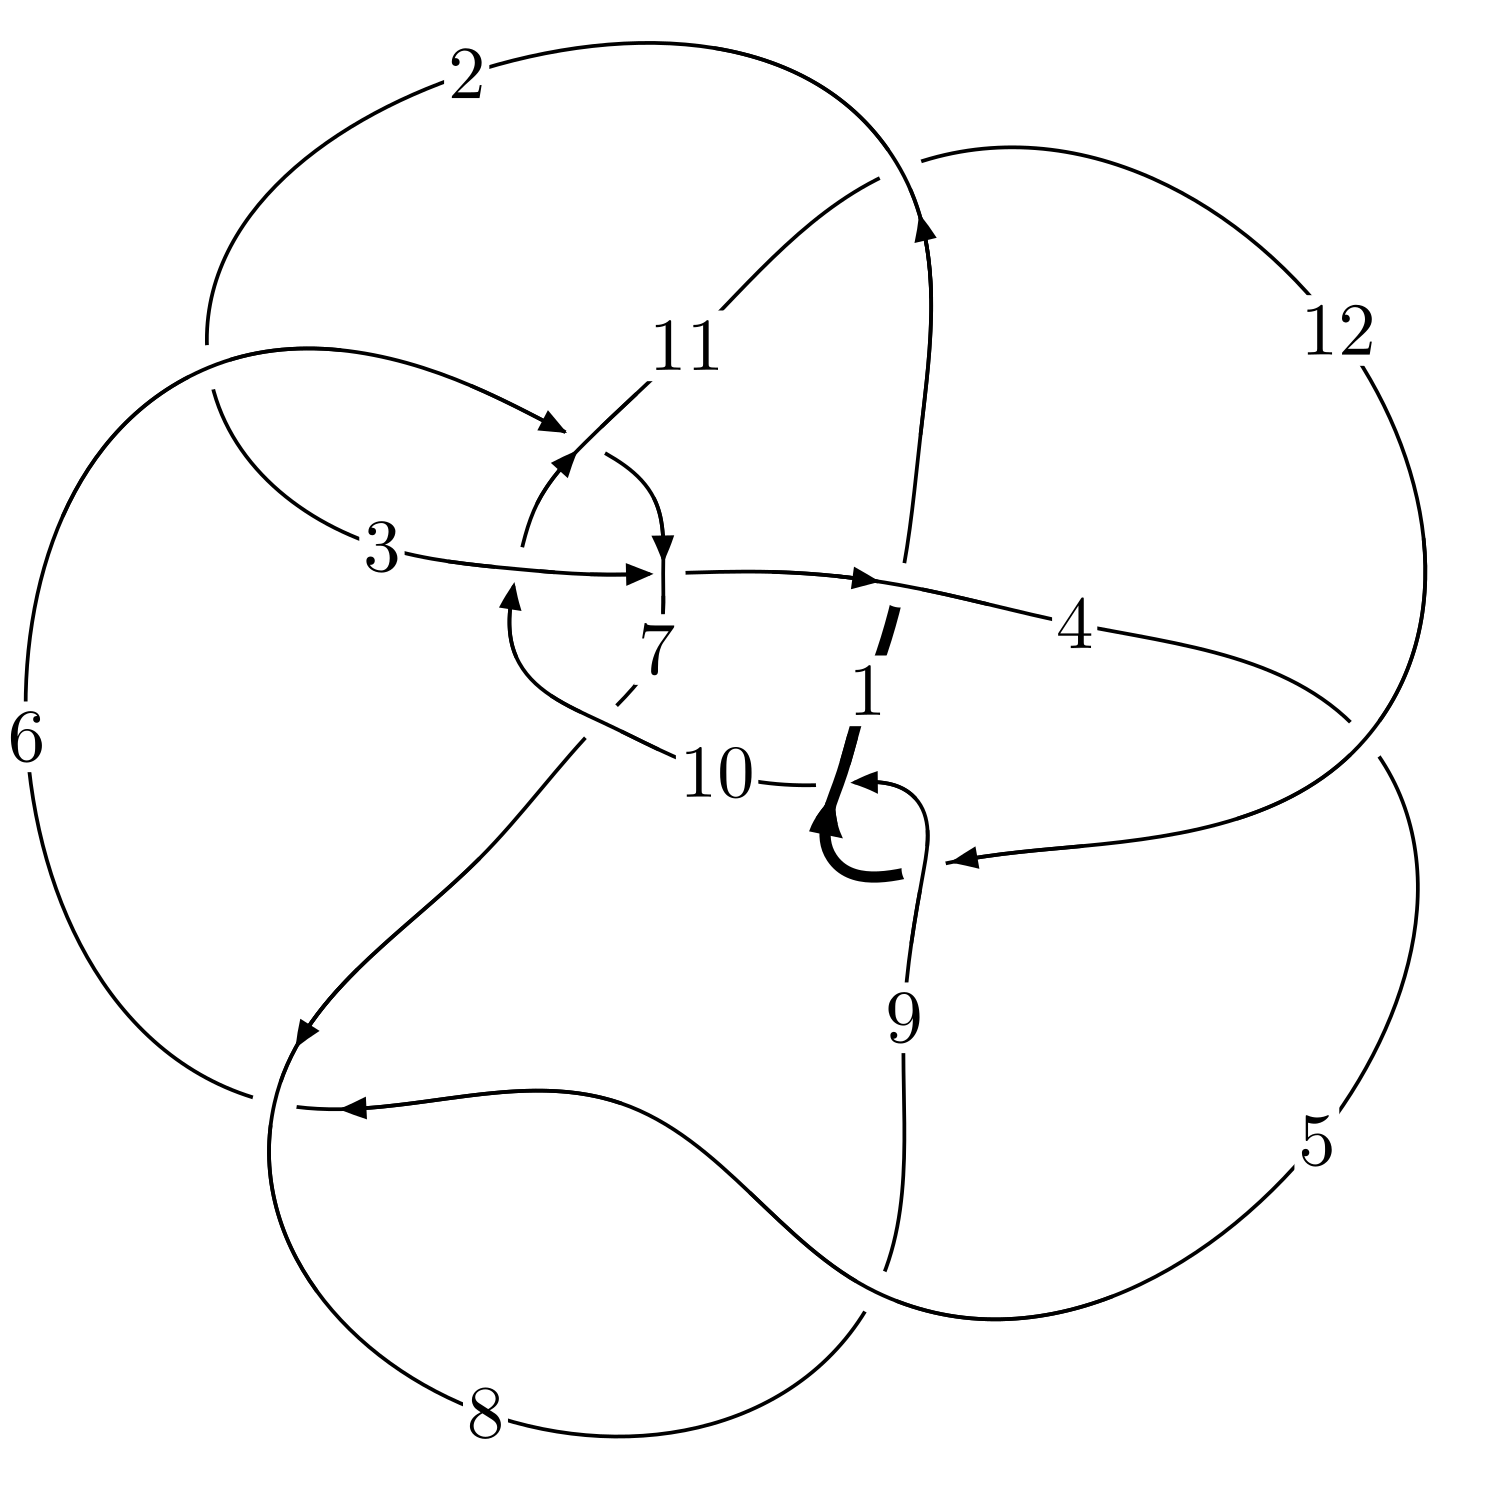
\includegraphics[width=112pt]{../../../GIT/diagram.site/Diagrams/png/1686_12a_0885.png}\\
\ \ \ A knot diagram\footnotemark}&
\allowdisplaybreaks
\textbf{Linearized knot diagam} \\
\cline{2-2}
 &
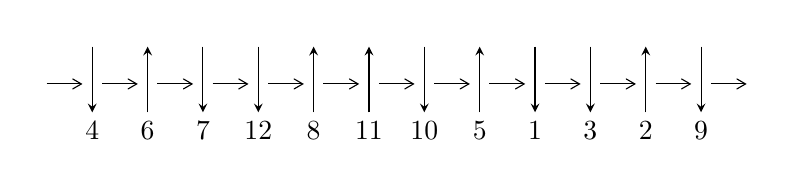
\begin{tikzpicture}[x=20pt, y=17pt]
	% nodes
	\node (C0) at (0, 0) {};
	\node (C1) at (1, 0) {};
	\node (C1U) at (1, +1) {};
	\node (C1D) at (1, -1) {4};

	\node (C2) at (2, 0) {};
	\node (C2U) at (2, +1) {};
	\node (C2D) at (2, -1) {6};

	\node (C3) at (3, 0) {};
	\node (C3U) at (3, +1) {};
	\node (C3D) at (3, -1) {7};

	\node (C4) at (4, 0) {};
	\node (C4U) at (4, +1) {};
	\node (C4D) at (4, -1) {12};

	\node (C5) at (5, 0) {};
	\node (C5U) at (5, +1) {};
	\node (C5D) at (5, -1) {8};

	\node (C6) at (6, 0) {};
	\node (C6U) at (6, +1) {};
	\node (C6D) at (6, -1) {11};

	\node (C7) at (7, 0) {};
	\node (C7U) at (7, +1) {};
	\node (C7D) at (7, -1) {10};

	\node (C8) at (8, 0) {};
	\node (C8U) at (8, +1) {};
	\node (C8D) at (8, -1) {5};

	\node (C9) at (9, 0) {};
	\node (C9U) at (9, +1) {};
	\node (C9D) at (9, -1) {1};

	\node (C10) at (10, 0) {};
	\node (C10U) at (10, +1) {};
	\node (C10D) at (10, -1) {3};

	\node (C11) at (11, 0) {};
	\node (C11U) at (11, +1) {};
	\node (C11D) at (11, -1) {2};

	\node (C12) at (12, 0) {};
	\node (C12U) at (12, +1) {};
	\node (C12D) at (12, -1) {9};
	\node (C13) at (13, 0) {};

	% arrows
	\draw[->,>={angle 60}]
	(C0) edge (C1) (C1) edge (C2) (C2) edge (C3) (C3) edge (C4) (C4) edge (C5) (C5) edge (C6) (C6) edge (C7) (C7) edge (C8) (C8) edge (C9) (C9) edge (C10) (C10) edge (C11) (C11) edge (C12) (C12) edge (C13) ;	\draw[->,>=stealth]
	(C1U) edge (C1D) (C2D) edge (C2U) (C3U) edge (C3D) (C4U) edge (C4D) (C5D) edge (C5U) (C6D) edge (C6U) (C7U) edge (C7D) (C8D) edge (C8U) (C9U) edge (C9D) (C10U) edge (C10D) (C11D) edge (C11U) (C12U) edge (C12D) ;
	\end{tikzpicture} \\
\hhline{~~} \\& 
\textbf{Solving Sequence} \\ \cline{2-2} 
 &
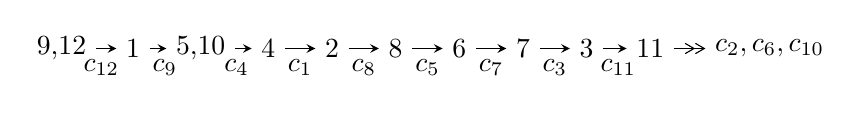
\begin{tikzpicture}[x=23pt, y=7pt]
	% node
	\node (A0) at (-1/8, 0) {9,12};
	\node (A1) at (1, 0) {1};
	\node (A2) at (33/16, 0) {5,10};
	\node (A3) at (25/8, 0) {4};
	\node (A4) at (33/8, 0) {2};
	\node (A5) at (41/8, 0) {8};
	\node (A6) at (49/8, 0) {6};
	\node (A7) at (57/8, 0) {7};
	\node (A8) at (65/8, 0) {3};
	\node (A9) at (73/8, 0) {11};
	\node (C1) at (1/2, -1) {$c_{12}$};
	\node (C2) at (3/2, -1) {$c_{9}$};
	\node (C3) at (21/8, -1) {$c_{4}$};
	\node (C4) at (29/8, -1) {$c_{1}$};
	\node (C5) at (37/8, -1) {$c_{8}$};
	\node (C6) at (45/8, -1) {$c_{5}$};
	\node (C7) at (53/8, -1) {$c_{7}$};
	\node (C8) at (61/8, -1) {$c_{3}$};
	\node (C9) at (69/8, -1) {$c_{11}$};
	\node (A10) at (11, 0) {$c_{2},c_{6},c_{10}$};

	% edge
	\draw[->,>=stealth]	
	(A0) edge (A1) (A1) edge (A2) (A2) edge (A3) (A3) edge (A4) (A4) edge (A5) (A5) edge (A6) (A6) edge (A7) (A7) edge (A8) (A8) edge (A9) ;
	\draw[->>,>={angle 60}]	
	(A9) edge (A10);
\end{tikzpicture} \\ 

\end{tabular} \\

\footnotetext{
The image of knot diagram is generated by the software ``\textbf{Draw programme}" developed by Andrew Bartholomew(\url{http://www.layer8.co.uk/maths/draw/index.htm\#Running-draw}), where we modified some parts for our purpose(\url{https://github.com/CATsTAILs/LinksPainter}).
}\phantom \\ \newline 
\centering \textbf{Ideals for irreducible components\footnotemark of $X_{\text{par}}$} 
 
\begin{align*}
I^u_{1}&=\langle 
-4.52853\times10^{1348} u^{191}-4.40776\times10^{1348} u^{190}+\cdots+3.02536\times10^{1349} b+8.87488\times10^{1353},\\
\phantom{I^u_{1}}&\phantom{= \langle  }5.55369\times10^{1354} u^{191}+6.03965\times10^{1354} u^{190}+\cdots+5.77581\times10^{1354} a-9.76561\times10^{1359},\\
\phantom{I^u_{1}}&\phantom{= \langle  }u^{192}-66 u^{190}+\cdots-260505 u+190913\rangle \\
I^u_{2}&=\langle 
-2.32335\times10^{58} u^{45}+9.00536\times10^{58} u^{44}+\cdots+5.08445\times10^{58} b-2.32363\times10^{58},\\
\phantom{I^u_{2}}&\phantom{= \langle  }8.57429\times10^{57} u^{45}-6.83963\times10^{58} u^{44}+\cdots+5.08445\times10^{58} a-1.60246\times10^{59},\;u^{46}- u^{45}+\cdots+4 u+1\rangle \\
I^u_{3}&=\langle 
u^2+b-1,\;a,\;u^3- u+1\rangle \\
\\
\end{align*}
\raggedright * 3 irreducible components of $\dim_{\mathbb{C}}=0$, with total 241 representations.\\
\footnotetext{All coefficients of polynomials are rational numbers. But the coefficients are sometimes approximated in decimal forms when there is not enough margin.}
\newpage
\renewcommand{\arraystretch}{1}
\centering \section*{I. $I^u_{1}= \langle -4.53\times10^{1348} u^{191}-4.41\times10^{1348} u^{190}+\cdots+3.03\times10^{1349} b+8.87\times10^{1353},\;5.55\times10^{1354} u^{191}+6.04\times10^{1354} u^{190}+\cdots+5.78\times10^{1354} a-9.77\times10^{1359},\;u^{192}-66 u^{190}+\cdots-260505 u+190913 \rangle$}
\flushleft \textbf{(i) Arc colorings}\\
\begin{tabular}{m{7pt} m{180pt} m{7pt} m{180pt} }
\flushright $a_{9}=$&$\begin{pmatrix}0\\u\end{pmatrix}$ \\
\flushright $a_{12}=$&$\begin{pmatrix}1\\0\end{pmatrix}$ \\
\flushright $a_{1}=$&$\begin{pmatrix}1\\u^2\end{pmatrix}$ \\
\flushright $a_{5}=$&$\begin{pmatrix}-0.961543 u^{191}-1.04568 u^{190}+\cdots-75031.1 u+169078.\\0.149686 u^{191}+0.145693 u^{190}+\cdots+10084.4 u-29334.9\end{pmatrix}$ \\
\flushright $a_{10}=$&$\begin{pmatrix}- u\\- u^3+u\end{pmatrix}$ \\
\flushright $a_{4}=$&$\begin{pmatrix}-0.811857 u^{191}-0.899986 u^{190}+\cdots-64946.7 u+139743.\\0.149686 u^{191}+0.145693 u^{190}+\cdots+10084.4 u-29334.9\end{pmatrix}$ \\
\flushright $a_{2}=$&$\begin{pmatrix}1.53091 u^{191}+1.69422 u^{190}+\cdots+121583. u-264246.\\0.260752 u^{191}+0.286880 u^{190}+\cdots+20365.1 u-45511.1\end{pmatrix}$ \\
\flushright $a_{8}=$&$\begin{pmatrix}1.10499 u^{191}+1.22263 u^{190}+\cdots+88020.6 u-190738.\\0.139490 u^{191}+0.165249 u^{190}+\cdots+11817.1 u-22474.1\end{pmatrix}$ \\
\flushright $a_{6}=$&$\begin{pmatrix}3.00511 u^{191}+3.25714 u^{190}+\cdots+233858. u-529065.\\0.0344419 u^{191}+0.0295635 u^{190}+\cdots+2010.33 u-7319.91\end{pmatrix}$ \\
\flushright $a_{7}=$&$\begin{pmatrix}0.998536 u^{191}+1.11888 u^{190}+\cdots+80578.5 u-170226.\\0.146191 u^{191}+0.175037 u^{190}+\cdots+12554.3 u-23179.0\end{pmatrix}$ \\
\flushright $a_{3}=$&$\begin{pmatrix}-0.222952 u^{191}-0.268722 u^{190}+\cdots-19410.7 u+34741.5\\-0.628421 u^{191}-0.691947 u^{190}+\cdots-49938.6 u+108743.\end{pmatrix}$ \\
\flushright $a_{11}=$&$\begin{pmatrix}3.38660 u^{191}+3.68537 u^{190}+\cdots+264761. u-593916.\\0.724951 u^{191}+0.791999 u^{190}+\cdots+57418.1 u-126129.\end{pmatrix}$\\&\end{tabular}
\flushleft \textbf{(ii) Obstruction class $= -1$}\\~\\
\flushleft \textbf{(iii) Cusp Shapes $= -7.52882 u^{191}-7.76256 u^{190}+\cdots-547014. u+1.39459\times10^{6}$}\\~\\
\newpage\renewcommand{\arraystretch}{1}
\flushleft \textbf{(iv) u-Polynomials at the component}\newline \\
\begin{tabular}{m{50pt}|m{274pt}}
Crossings & \hspace{64pt}u-Polynomials at each crossing \\
\hline $$\begin{aligned}c_{1}\end{aligned}$$&$\begin{aligned}
&u^{192}+11 u^{191}+\cdots+11366 u-13097
\end{aligned}$\\
\hline $$\begin{aligned}c_{2}\end{aligned}$$&$\begin{aligned}
&u^{192}+12 u^{190}+\cdots+43 u+1
\end{aligned}$\\
\hline $$\begin{aligned}c_{3}\end{aligned}$$&$\begin{aligned}
&u^{192}+6 u^{191}+\cdots+162 u-81
\end{aligned}$\\
\hline $$\begin{aligned}c_{4}\end{aligned}$$&$\begin{aligned}
&u^{192}+u^{191}+\cdots+34724083357 u-1929655883
\end{aligned}$\\
\hline $$\begin{aligned}c_{5},c_{8}\end{aligned}$$&$\begin{aligned}
&u^{192}-7 u^{191}+\cdots-54816024 u+2680568
\end{aligned}$\\
\hline $$\begin{aligned}c_{6}\end{aligned}$$&$\begin{aligned}
&u^{192}-3 u^{191}+\cdots+145 u+7
\end{aligned}$\\
\hline $$\begin{aligned}c_{7}\end{aligned}$$&$\begin{aligned}
&u^{192}-15 u^{191}+\cdots-288765 u+40025
\end{aligned}$\\
\hline $$\begin{aligned}c_{9},c_{12}\end{aligned}$$&$\begin{aligned}
&u^{192}-66 u^{190}+\cdots+260505 u+190913
\end{aligned}$\\
\hline $$\begin{aligned}c_{10}\end{aligned}$$&$\begin{aligned}
&u^{192}+u^{191}+\cdots+67 u+11
\end{aligned}$\\
\hline $$\begin{aligned}c_{11}\end{aligned}$$&$\begin{aligned}
&u^{192}+13 u^{191}+\cdots-447056 u+393584
\end{aligned}$\\
\hline
\end{tabular}\\~\\
\newpage\renewcommand{\arraystretch}{1}
\flushleft \textbf{(v) Riley Polynomials at the component}\newline \\
\begin{tabular}{m{50pt}|m{274pt}}
Crossings & \hspace{64pt}Riley Polynomials at each crossing \\
\hline $$\begin{aligned}c_{1}\end{aligned}$$&$\begin{aligned}
&y^{192}-19 y^{191}+\cdots-5625892080 y+171531409
\end{aligned}$\\
\hline $$\begin{aligned}c_{2}\end{aligned}$$&$\begin{aligned}
&y^{192}+24 y^{191}+\cdots-25 y+1
\end{aligned}$\\
\hline $$\begin{aligned}c_{3}\end{aligned}$$&$\begin{aligned}
&y^{192}+8 y^{191}+\cdots+4694760 y+6561
\end{aligned}$\\
\hline $$\begin{aligned}c_{4}\end{aligned}$$&$\begin{aligned}
&y^{192}-57 y^{191}+\cdots-3.74\times10^{20} y+3.72\times10^{18}
\end{aligned}$\\
\hline $$\begin{aligned}c_{5},c_{8}\end{aligned}$$&$\begin{aligned}
&y^{192}+159 y^{191}+\cdots-1182090996599008 y+7185444802624
\end{aligned}$\\
\hline $$\begin{aligned}c_{6}\end{aligned}$$&$\begin{aligned}
&y^{192}+27 y^{191}+\cdots+4161 y+49
\end{aligned}$\\
\hline $$\begin{aligned}c_{7}\end{aligned}$$&$\begin{aligned}
&y^{192}+11 y^{191}+\cdots+28375301475 y+1602000625
\end{aligned}$\\
\hline $$\begin{aligned}c_{9},c_{12}\end{aligned}$$&$\begin{aligned}
&y^{192}-132 y^{191}+\cdots-2163961974271 y+36447773569
\end{aligned}$\\
\hline $$\begin{aligned}c_{10}\end{aligned}$$&$\begin{aligned}
&y^{192}-5 y^{191}+\cdots-37181 y+121
\end{aligned}$\\
\hline $$\begin{aligned}c_{11}\end{aligned}$$&$\begin{aligned}
&y^{192}+51 y^{191}+\cdots+17097698026752 y+154908365056
\end{aligned}$\\
\hline
\end{tabular}\\~\\
\newpage\flushleft \textbf{(vi) Complex Volumes and Cusp Shapes}
$$\begin{array}{c|c|c}  
\text{Solutions to }I^u_{1}& \I (\text{vol} + \sqrt{-1}CS) & \text{Cusp shape}\\
 \hline 
\begin{aligned}
u &= -0.305368 + 0.942192 I \\
a &= \phantom{-}0.110413 - 0.540846 I \\
b &= \phantom{-}0.090117 + 0.706383 I\end{aligned}
 & \phantom{-}4.07931 - 2.76969 I & \phantom{-0.000000 } 0 \\ \hline\begin{aligned}
u &= -0.305368 - 0.942192 I \\
a &= \phantom{-}0.110413 + 0.540846 I \\
b &= \phantom{-}0.090117 - 0.706383 I\end{aligned}
 & \phantom{-}4.07931 + 2.76969 I & \phantom{-0.000000 } 0 \\ \hline\begin{aligned}
u &= \phantom{-}0.867048 + 0.469921 I \\
a &= -0.363887 - 0.862845 I \\
b &= \phantom{-}1.56487 - 0.08295 I\end{aligned}
 & -2.39773 - 0.74504 I & \phantom{-0.000000 } 0 \\ \hline\begin{aligned}
u &= \phantom{-}0.867048 - 0.469921 I \\
a &= -0.363887 + 0.862845 I \\
b &= \phantom{-}1.56487 + 0.08295 I\end{aligned}
 & -2.39773 + 0.74504 I & \phantom{-0.000000 } 0 \\ \hline\begin{aligned}
u &= \phantom{-}0.481447 + 0.859612 I \\
a &= -0.358476 - 0.689493 I \\
b &= -0.186779 + 0.743677 I\end{aligned}
 & \phantom{-}3.17644 - 5.60653 I & \phantom{-0.000000 } 0 \\ \hline\begin{aligned}
u &= \phantom{-}0.481447 - 0.859612 I \\
a &= -0.358476 + 0.689493 I \\
b &= -0.186779 - 0.743677 I\end{aligned}
 & \phantom{-}3.17644 + 5.60653 I & \phantom{-0.000000 } 0 \\ \hline\begin{aligned}
u &= \phantom{-}0.159304 + 0.965248 I \\
a &= \phantom{-}0.492221 + 0.736064 I \\
b &= -0.547287 - 0.604217 I\end{aligned}
 & \phantom{-}1.57080 - 4.06752 I & \phantom{-0.000000 } 0 \\ \hline\begin{aligned}
u &= \phantom{-}0.159304 - 0.965248 I \\
a &= \phantom{-}0.492221 - 0.736064 I \\
b &= -0.547287 + 0.604217 I\end{aligned}
 & \phantom{-}1.57080 + 4.06752 I & \phantom{-0.000000 } 0 \\ \hline\begin{aligned}
u &= \phantom{-}0.970622 + 0.078100 I \\
a &= -0.036052 - 1.139680 I \\
b &= \phantom{-}2.15368 + 2.31038 I\end{aligned}
 & -3.20206 - 2.23235 I & \phantom{-0.000000 } 0 \\ \hline\begin{aligned}
u &= \phantom{-}0.970622 - 0.078100 I \\
a &= -0.036052 + 1.139680 I \\
b &= \phantom{-}2.15368 - 2.31038 I\end{aligned}
 & -3.20206 + 2.23235 I & \phantom{-0.000000 } 0\\
 \hline 
 \end{array}$$\newpage$$\begin{array}{c|c|c}  
\text{Solutions to }I^u_{1}& \I (\text{vol} + \sqrt{-1}CS) & \text{Cusp shape}\\
 \hline 
\begin{aligned}
u &= -0.974854 + 0.339727 I \\
a &= \phantom{-}0.526466 + 1.165590 I \\
b &= \phantom{-}1.158080 - 0.784931 I\end{aligned}
 & \phantom{-}0.16374 + 4.64361 I & \phantom{-0.000000 } 0 \\ \hline\begin{aligned}
u &= -0.974854 - 0.339727 I \\
a &= \phantom{-}0.526466 - 1.165590 I \\
b &= \phantom{-}1.158080 + 0.784931 I\end{aligned}
 & \phantom{-}0.16374 - 4.64361 I & \phantom{-0.000000 } 0 \\ \hline\begin{aligned}
u &= \phantom{-}0.238694 + 1.011990 I \\
a &= -1.297170 + 0.056141 I \\
b &= \phantom{-}1.186040 - 0.534383 I\end{aligned}
 & -2.43406 + 6.12195 I & \phantom{-0.000000 } 0 \\ \hline\begin{aligned}
u &= \phantom{-}0.238694 - 1.011990 I \\
a &= -1.297170 - 0.056141 I \\
b &= \phantom{-}1.186040 + 0.534383 I\end{aligned}
 & -2.43406 - 6.12195 I & \phantom{-0.000000 } 0 \\ \hline\begin{aligned}
u &= \phantom{-}0.305304 + 0.908849 I \\
a &= -1.028910 - 0.696941 I \\
b &= \phantom{-}1.090190 + 0.526989 I\end{aligned}
 & -3.94137 - 3.92448 I & \phantom{-0.000000 } 0 \\ \hline\begin{aligned}
u &= \phantom{-}0.305304 - 0.908849 I \\
a &= -1.028910 + 0.696941 I \\
b &= \phantom{-}1.090190 - 0.526989 I\end{aligned}
 & -3.94137 + 3.92448 I & \phantom{-0.000000 } 0 \\ \hline\begin{aligned}
u &= \phantom{-}0.943288 + 0.165892 I \\
a &= \phantom{-}0.24864 + 2.25461 I \\
b &= -0.614650 - 0.455829 I\end{aligned}
 & -5.25118 - 5.63591 I & \phantom{-0.000000 } 0 \\ \hline\begin{aligned}
u &= \phantom{-}0.943288 - 0.165892 I \\
a &= \phantom{-}0.24864 - 2.25461 I \\
b &= -0.614650 + 0.455829 I\end{aligned}
 & -5.25118 + 5.63591 I & \phantom{-0.000000 } 0 \\ \hline\begin{aligned}
u &= \phantom{-}1.042920 + 0.039723 I \\
a &= -0.069996 - 1.059350 I \\
b &= -1.68735 + 3.57633 I\end{aligned}
 & -3.39563 - 2.19088 I & \phantom{-0.000000 } 0 \\ \hline\begin{aligned}
u &= \phantom{-}1.042920 - 0.039723 I \\
a &= -0.069996 + 1.059350 I \\
b &= -1.68735 - 3.57633 I\end{aligned}
 & -3.39563 + 2.19088 I & \phantom{-0.000000 } 0\\
 \hline 
 \end{array}$$\newpage$$\begin{array}{c|c|c}  
\text{Solutions to }I^u_{1}& \I (\text{vol} + \sqrt{-1}CS) & \text{Cusp shape}\\
 \hline 
\begin{aligned}
u &= -0.935948 + 0.517165 I \\
a &= -0.645535 + 0.204146 I \\
b &= \phantom{-}0.94217 + 1.10518 I\end{aligned}
 & -1.26562 + 8.71875 I & \phantom{-0.000000 } 0 \\ \hline\begin{aligned}
u &= -0.935948 - 0.517165 I \\
a &= -0.645535 - 0.204146 I \\
b &= \phantom{-}0.94217 - 1.10518 I\end{aligned}
 & -1.26562 - 8.71875 I & \phantom{-0.000000 } 0 \\ \hline\begin{aligned}
u &= \phantom{-}0.069314 + 1.089720 I \\
a &= -1.110850 + 0.091728 I \\
b &= \phantom{-}0.989033 + 0.287582 I\end{aligned}
 & -3.01334 - 0.11433 I & \phantom{-0.000000 } 0 \\ \hline\begin{aligned}
u &= \phantom{-}0.069314 - 1.089720 I \\
a &= -1.110850 - 0.091728 I \\
b &= \phantom{-}0.989033 - 0.287582 I\end{aligned}
 & -3.01334 + 0.11433 I & \phantom{-0.000000 } 0 \\ \hline\begin{aligned}
u &= \phantom{-}0.769753 + 0.479609 I \\
a &= -0.283950 + 0.796787 I \\
b &= -0.231751 + 0.208273 I\end{aligned}
 & -0.51327 - 2.35678 I & \phantom{-0.000000 } 0 \\ \hline\begin{aligned}
u &= \phantom{-}0.769753 - 0.479609 I \\
a &= -0.283950 - 0.796787 I \\
b &= -0.231751 - 0.208273 I\end{aligned}
 & -0.51327 + 2.35678 I & \phantom{-0.000000 } 0 \\ \hline\begin{aligned}
u &= \phantom{-}1.094820 + 0.007773 I \\
a &= \phantom{-}0.72992 - 2.16327 I \\
b &= \phantom{-}0.562751 + 0.193330 I\end{aligned}
 & -6.21148 + 5.06576 I & \phantom{-0.000000 } 0 \\ \hline\begin{aligned}
u &= \phantom{-}1.094820 - 0.007773 I \\
a &= \phantom{-}0.72992 + 2.16327 I \\
b &= \phantom{-}0.562751 - 0.193330 I\end{aligned}
 & -6.21148 - 5.06576 I & \phantom{-0.000000 } 0 \\ \hline\begin{aligned}
u &= -1.086090 + 0.146403 I \\
a &= -0.087948 - 1.053020 I \\
b &= \phantom{-}0.22516 + 2.39185 I\end{aligned}
 & -3.14940 + 11.56240 I & \phantom{-0.000000 } 0 \\ \hline\begin{aligned}
u &= -1.086090 - 0.146403 I \\
a &= -0.087948 + 1.053020 I \\
b &= \phantom{-}0.22516 - 2.39185 I\end{aligned}
 & -3.14940 - 11.56240 I & \phantom{-0.000000 } 0\\
 \hline 
 \end{array}$$\newpage$$\begin{array}{c|c|c}  
\text{Solutions to }I^u_{1}& \I (\text{vol} + \sqrt{-1}CS) & \text{Cusp shape}\\
 \hline 
\begin{aligned}
u &= -0.899444 + 0.054586 I \\
a &= \phantom{-}0.284465 + 1.110460 I \\
b &= \phantom{-}0.48414 - 1.40464 I\end{aligned}
 & \phantom{-}0.49587 + 3.42536 I & \phantom{-0.000000 } 0 \\ \hline\begin{aligned}
u &= -0.899444 - 0.054586 I \\
a &= \phantom{-}0.284465 - 1.110460 I \\
b &= \phantom{-}0.48414 + 1.40464 I\end{aligned}
 & \phantom{-}0.49587 - 3.42536 I & \phantom{-0.000000 } 0 \\ \hline\begin{aligned}
u &= -0.796022 + 0.759997 I \\
a &= \phantom{-}0.487024 - 0.914704 I \\
b &= -1.52510 - 0.02964 I\end{aligned}
 & -1.12884 + 8.61985 I & \phantom{-0.000000 } 0 \\ \hline\begin{aligned}
u &= -0.796022 - 0.759997 I \\
a &= \phantom{-}0.487024 + 0.914704 I \\
b &= -1.52510 + 0.02964 I\end{aligned}
 & -1.12884 - 8.61985 I & \phantom{-0.000000 } 0 \\ \hline\begin{aligned}
u &= -0.993985 + 0.477806 I \\
a &= \phantom{-}0.545470 - 1.274570 I \\
b &= -1.101560 + 0.254031 I\end{aligned}
 & -7.28880 - 2.65302 I & \phantom{-0.000000 } 0 \\ \hline\begin{aligned}
u &= -0.993985 - 0.477806 I \\
a &= \phantom{-}0.545470 + 1.274570 I \\
b &= -1.101560 - 0.254031 I\end{aligned}
 & -7.28880 + 2.65302 I & \phantom{-0.000000 } 0 \\ \hline\begin{aligned}
u &= \phantom{-}1.058770 + 0.309676 I \\
a &= -1.144730 + 0.666006 I \\
b &= -1.036080 - 0.737442 I\end{aligned}
 & -0.13894 - 5.07779 I & \phantom{-0.000000 } 0 \\ \hline\begin{aligned}
u &= \phantom{-}1.058770 - 0.309676 I \\
a &= -1.144730 - 0.666006 I \\
b &= -1.036080 + 0.737442 I\end{aligned}
 & -0.13894 + 5.07779 I & \phantom{-0.000000 } 0 \\ \hline\begin{aligned}
u &= \phantom{-}1.107260 + 0.067096 I \\
a &= -0.285398 + 1.107910 I \\
b &= -0.05333 - 2.07988 I\end{aligned}
 & -2.35852 - 2.75429 I & \phantom{-0.000000 } 0 \\ \hline\begin{aligned}
u &= \phantom{-}1.107260 - 0.067096 I \\
a &= -0.285398 - 1.107910 I \\
b &= -0.05333 + 2.07988 I\end{aligned}
 & -2.35852 + 2.75429 I & \phantom{-0.000000 } 0\\
 \hline 
 \end{array}$$\newpage$$\begin{array}{c|c|c}  
\text{Solutions to }I^u_{1}& \I (\text{vol} + \sqrt{-1}CS) & \text{Cusp shape}\\
 \hline 
\begin{aligned}
u &= \phantom{-}0.312180 + 0.827366 I \\
a &= \phantom{-}1.50708 + 0.67486 I \\
b &= -0.905828 - 0.573173 I\end{aligned}
 & -5.17128 - 6.53541 I & \phantom{-0.000000 } 0 \\ \hline\begin{aligned}
u &= \phantom{-}0.312180 - 0.827366 I \\
a &= \phantom{-}1.50708 - 0.67486 I \\
b &= -0.905828 + 0.573173 I\end{aligned}
 & -5.17128 + 6.53541 I & \phantom{-0.000000 } 0 \\ \hline\begin{aligned}
u &= \phantom{-}0.874586 + 0.112468 I \\
a &= -0.469015 + 0.973330 I \\
b &= -2.37603 + 1.42021 I\end{aligned}
 & -1.23213 - 2.20378 I & \phantom{-0.000000 } 0 \\ \hline\begin{aligned}
u &= \phantom{-}0.874586 - 0.112468 I \\
a &= -0.469015 - 0.973330 I \\
b &= -2.37603 - 1.42021 I\end{aligned}
 & -1.23213 + 2.20378 I & \phantom{-0.000000 } 0 \\ \hline\begin{aligned}
u &= \phantom{-}1.063830 + 0.346254 I \\
a &= -0.115968 - 0.301971 I \\
b &= \phantom{-}0.856147 - 0.146668 I\end{aligned}
 & -2.02076 - 0.56587 I & \phantom{-0.000000 } 0 \\ \hline\begin{aligned}
u &= \phantom{-}1.063830 - 0.346254 I \\
a &= -0.115968 + 0.301971 I \\
b &= \phantom{-}0.856147 + 0.146668 I\end{aligned}
 & -2.02076 + 0.56587 I & \phantom{-0.000000 } 0 \\ \hline\begin{aligned}
u &= \phantom{-}0.803548 + 0.353842 I \\
a &= \phantom{-}0.211760 + 0.419784 I \\
b &= -0.607727 + 1.241630 I\end{aligned}
 & -1.72811 - 2.09926 I & \phantom{-0.000000 } 0 \\ \hline\begin{aligned}
u &= \phantom{-}0.803548 - 0.353842 I \\
a &= \phantom{-}0.211760 - 0.419784 I \\
b &= -0.607727 - 1.241630 I\end{aligned}
 & -1.72811 + 2.09926 I & \phantom{-0.000000 } 0 \\ \hline\begin{aligned}
u &= \phantom{-}1.133420 + 0.025545 I \\
a &= -0.447167 + 0.543690 I \\
b &= -1.21044 + 0.73880 I\end{aligned}
 & -3.67970 + 1.40620 I & \phantom{-0.000000 } 0 \\ \hline\begin{aligned}
u &= \phantom{-}1.133420 - 0.025545 I \\
a &= -0.447167 - 0.543690 I \\
b &= -1.21044 - 0.73880 I\end{aligned}
 & -3.67970 - 1.40620 I & \phantom{-0.000000 } 0\\
 \hline 
 \end{array}$$\newpage$$\begin{array}{c|c|c}  
\text{Solutions to }I^u_{1}& \I (\text{vol} + \sqrt{-1}CS) & \text{Cusp shape}\\
 \hline 
\begin{aligned}
u &= -1.132390 + 0.085969 I \\
a &= \phantom{-}0.17312 + 1.48786 I \\
b &= \phantom{-}1.064260 - 0.632811 I\end{aligned}
 & -8.47850 + 4.57950 I & \phantom{-0.000000 } 0 \\ \hline\begin{aligned}
u &= -1.132390 - 0.085969 I \\
a &= \phantom{-}0.17312 - 1.48786 I \\
b &= \phantom{-}1.064260 + 0.632811 I\end{aligned}
 & -8.47850 - 4.57950 I & \phantom{-0.000000 } 0 \\ \hline\begin{aligned}
u &= -1.124730 + 0.173697 I \\
a &= -0.141884 + 1.209500 I \\
b &= -0.106376 - 1.113790 I\end{aligned}
 & -3.53497 + 4.99188 I & \phantom{-0.000000 } 0 \\ \hline\begin{aligned}
u &= -1.124730 - 0.173697 I \\
a &= -0.141884 - 1.209500 I \\
b &= -0.106376 + 1.113790 I\end{aligned}
 & -3.53497 - 4.99188 I & \phantom{-0.000000 } 0 \\ \hline\begin{aligned}
u &= -0.809277 + 0.288353 I \\
a &= \phantom{-}0.954266 + 0.733731 I \\
b &= \phantom{-}0.392319 - 0.327849 I\end{aligned}
 & \phantom{-}1.54455 + 1.72701 I & \phantom{-0.000000 } 0 \\ \hline\begin{aligned}
u &= -0.809277 - 0.288353 I \\
a &= \phantom{-}0.954266 - 0.733731 I \\
b &= \phantom{-}0.392319 + 0.327849 I\end{aligned}
 & \phantom{-}1.54455 - 1.72701 I & \phantom{-0.000000 } 0 \\ \hline\begin{aligned}
u &= -0.635234 + 0.570049 I \\
a &= \phantom{-}0.522799 + 0.792351 I \\
b &= \phantom{-}0.022074 - 0.888954 I\end{aligned}
 & \phantom{-}2.03268 + 2.00343 I & \phantom{-0.000000 } 0 \\ \hline\begin{aligned}
u &= -0.635234 - 0.570049 I \\
a &= \phantom{-}0.522799 - 0.792351 I \\
b &= \phantom{-}0.022074 + 0.888954 I\end{aligned}
 & \phantom{-}2.03268 - 2.00343 I & \phantom{-0.000000 } 0 \\ \hline\begin{aligned}
u &= \phantom{-}1.064340 + 0.468005 I \\
a &= \phantom{-}0.723498 - 0.029467 I \\
b &= \phantom{-}0.751564 + 0.213637 I\end{aligned}
 & \phantom{-}1.24268 + 0.84125 I & \phantom{-0.000000 } 0 \\ \hline\begin{aligned}
u &= \phantom{-}1.064340 - 0.468005 I \\
a &= \phantom{-}0.723498 + 0.029467 I \\
b &= \phantom{-}0.751564 - 0.213637 I\end{aligned}
 & \phantom{-}1.24268 - 0.84125 I & \phantom{-0.000000 } 0\\
 \hline 
 \end{array}$$\newpage$$\begin{array}{c|c|c}  
\text{Solutions to }I^u_{1}& \I (\text{vol} + \sqrt{-1}CS) & \text{Cusp shape}\\
 \hline 
\begin{aligned}
u &= \phantom{-}1.164350 + 0.058481 I \\
a &= -0.050434 + 0.695042 I \\
b &= \phantom{-}1.24526 - 1.49451 I\end{aligned}
 & -2.65715 - 1.57082 I & \phantom{-0.000000 } 0 \\ \hline\begin{aligned}
u &= \phantom{-}1.164350 - 0.058481 I \\
a &= -0.050434 - 0.695042 I \\
b &= \phantom{-}1.24526 + 1.49451 I\end{aligned}
 & -2.65715 + 1.57082 I & \phantom{-0.000000 } 0 \\ \hline\begin{aligned}
u &= -0.157356 + 0.812635 I \\
a &= \phantom{-}1.62829 - 0.44953 I \\
b &= -1.101990 + 0.371276 I\end{aligned}
 & -6.47800 - 2.03822 I & \phantom{-0.000000 } 0 \\ \hline\begin{aligned}
u &= -0.157356 - 0.812635 I \\
a &= \phantom{-}1.62829 + 0.44953 I \\
b &= -1.101990 - 0.371276 I\end{aligned}
 & -6.47800 + 2.03822 I & \phantom{-0.000000 } 0 \\ \hline\begin{aligned}
u &= -1.118270 + 0.356984 I \\
a &= \phantom{-}1.053190 + 0.818883 I \\
b &= \phantom{-}0.838701 - 0.716389 I\end{aligned}
 & \phantom{-}0.26808 + 5.86406 I & \phantom{-0.000000 } 0 \\ \hline\begin{aligned}
u &= -1.118270 - 0.356984 I \\
a &= \phantom{-}1.053190 - 0.818883 I \\
b &= \phantom{-}0.838701 + 0.716389 I\end{aligned}
 & \phantom{-}0.26808 - 5.86406 I & \phantom{-0.000000 } 0 \\ \hline\begin{aligned}
u &= \phantom{-}0.020401 + 1.173750 I \\
a &= \phantom{-}1.140610 + 0.374143 I \\
b &= -1.000230 - 0.475762 I\end{aligned}
 & -1.65808 - 6.79976 I & \phantom{-0.000000 } 0 \\ \hline\begin{aligned}
u &= \phantom{-}0.020401 - 1.173750 I \\
a &= \phantom{-}1.140610 - 0.374143 I \\
b &= -1.000230 + 0.475762 I\end{aligned}
 & -1.65808 + 6.79976 I & \phantom{-0.000000 } 0 \\ \hline\begin{aligned}
u &= -0.701610 + 0.951889 I \\
a &= -0.715301 + 0.589225 I \\
b &= \phantom{-}1.297320 + 0.312962 I\end{aligned}
 & -0.72678 - 2.51797 I & \phantom{-0.000000 } 0 \\ \hline\begin{aligned}
u &= -0.701610 - 0.951889 I \\
a &= -0.715301 - 0.589225 I \\
b &= \phantom{-}1.297320 - 0.312962 I\end{aligned}
 & -0.72678 + 2.51797 I & \phantom{-0.000000 } 0\\
 \hline 
 \end{array}$$\newpage$$\begin{array}{c|c|c}  
\text{Solutions to }I^u_{1}& \I (\text{vol} + \sqrt{-1}CS) & \text{Cusp shape}\\
 \hline 
\begin{aligned}
u &= -1.175080 + 0.167165 I \\
a &= \phantom{-}0.09392 + 1.67341 I \\
b &= \phantom{-}0.531288 - 0.494076 I\end{aligned}
 & -4.31427 + 4.91419 I & \phantom{-0.000000 } 0 \\ \hline\begin{aligned}
u &= -1.175080 - 0.167165 I \\
a &= \phantom{-}0.09392 - 1.67341 I \\
b &= \phantom{-}0.531288 + 0.494076 I\end{aligned}
 & -4.31427 - 4.91419 I & \phantom{-0.000000 } 0 \\ \hline\begin{aligned}
u &= \phantom{-}0.451422 + 0.674552 I \\
a &= -0.232071 + 0.371080 I \\
b &= \phantom{-}0.808574 - 0.610049 I\end{aligned}
 & -0.01951 + 2.31296 I & \phantom{-0.000000 } 0 \\ \hline\begin{aligned}
u &= \phantom{-}0.451422 - 0.674552 I \\
a &= -0.232071 - 0.371080 I \\
b &= \phantom{-}0.808574 + 0.610049 I\end{aligned}
 & -0.01951 - 2.31296 I & \phantom{-0.000000 } 0 \\ \hline\begin{aligned}
u &= -0.633951 + 0.465512 I \\
a &= \phantom{-}1.322230 - 0.170725 I \\
b &= -0.427598 - 0.964768 I\end{aligned}
 & \phantom{-}1.26438 - 1.21230 I & \phantom{-0.000000 } 0 \\ \hline\begin{aligned}
u &= -0.633951 - 0.465512 I \\
a &= \phantom{-}1.322230 + 0.170725 I \\
b &= -0.427598 + 0.964768 I\end{aligned}
 & \phantom{-}1.26438 + 1.21230 I & \phantom{-0.000000 } 0 \\ \hline\begin{aligned}
u &= \phantom{-}1.146370 + 0.404217 I \\
a &= -0.666920 + 0.524426 I \\
b &= -1.243780 - 0.337708 I\end{aligned}
 & -2.31218 - 6.47981 I & \phantom{-0.000000 } 0 \\ \hline\begin{aligned}
u &= \phantom{-}1.146370 - 0.404217 I \\
a &= -0.666920 - 0.524426 I \\
b &= -1.243780 + 0.337708 I\end{aligned}
 & -2.31218 + 6.47981 I & \phantom{-0.000000 } 0 \\ \hline\begin{aligned}
u &= -1.217410 + 0.038052 I \\
a &= -0.987024 + 0.928998 I \\
b &= -0.836116 + 0.024849 I\end{aligned}
 & -6.30075 + 1.93071 I & \phantom{-0.000000 } 0 \\ \hline\begin{aligned}
u &= -1.217410 - 0.038052 I \\
a &= -0.987024 - 0.928998 I \\
b &= -0.836116 - 0.024849 I\end{aligned}
 & -6.30075 - 1.93071 I & \phantom{-0.000000 } 0\\
 \hline 
 \end{array}$$\newpage$$\begin{array}{c|c|c}  
\text{Solutions to }I^u_{1}& \I (\text{vol} + \sqrt{-1}CS) & \text{Cusp shape}\\
 \hline 
\begin{aligned}
u &= -1.195630 + 0.252592 I \\
a &= \phantom{-}1.229890 - 0.082937 I \\
b &= \phantom{-}0.778095 - 0.159143 I\end{aligned}
 & -0.84744 + 2.01085 I & \phantom{-0.000000 } 0 \\ \hline\begin{aligned}
u &= -1.195630 - 0.252592 I \\
a &= \phantom{-}1.229890 + 0.082937 I \\
b &= \phantom{-}0.778095 + 0.159143 I\end{aligned}
 & -0.84744 - 2.01085 I & \phantom{-0.000000 } 0 \\ \hline\begin{aligned}
u &= \phantom{-}1.221330 + 0.130605 I \\
a &= \phantom{-}1.016110 - 0.572027 I \\
b &= \phantom{-}0.888204 + 0.554345 I\end{aligned}
 & -4.46644 + 2.83668 I & \phantom{-0.000000 } 0 \\ \hline\begin{aligned}
u &= \phantom{-}1.221330 - 0.130605 I \\
a &= \phantom{-}1.016110 + 0.572027 I \\
b &= \phantom{-}0.888204 - 0.554345 I\end{aligned}
 & -4.46644 - 2.83668 I & \phantom{-0.000000 } 0 \\ \hline\begin{aligned}
u &= \phantom{-}0.225125 + 0.736868 I \\
a &= \phantom{-}0.277337 - 1.119630 I \\
b &= -0.695257 + 0.968927 I\end{aligned}
 & \phantom{-}1.23337 + 10.52490 I & \phantom{-0.000000 } 0 \\ \hline\begin{aligned}
u &= \phantom{-}0.225125 - 0.736868 I \\
a &= \phantom{-}0.277337 + 1.119630 I \\
b &= -0.695257 - 0.968927 I\end{aligned}
 & \phantom{-}1.23337 - 10.52490 I & \phantom{-0.000000 } 0 \\ \hline\begin{aligned}
u &= -0.764209 + 0.096980 I \\
a &= -0.964939 + 0.640567 I \\
b &= -1.291280 + 0.071409 I\end{aligned}
 & \phantom{-}0.37084 + 4.87903 I & \phantom{-0.000000 } 0 \\ \hline\begin{aligned}
u &= -0.764209 - 0.096980 I \\
a &= -0.964939 - 0.640567 I \\
b &= -1.291280 - 0.071409 I\end{aligned}
 & \phantom{-}0.37084 - 4.87903 I & \phantom{-0.000000 } 0 \\ \hline\begin{aligned}
u &= -1.233510 + 0.084242 I \\
a &= -0.708049 + 0.160514 I \\
b &= -1.026690 + 0.237295 I\end{aligned}
 & -5.79287 + 2.31865 I & \phantom{-0.000000 } 0 \\ \hline\begin{aligned}
u &= -1.233510 - 0.084242 I \\
a &= -0.708049 - 0.160514 I \\
b &= -1.026690 - 0.237295 I\end{aligned}
 & -5.79287 - 2.31865 I & \phantom{-0.000000 } 0\\
 \hline 
 \end{array}$$\newpage$$\begin{array}{c|c|c}  
\text{Solutions to }I^u_{1}& \I (\text{vol} + \sqrt{-1}CS) & \text{Cusp shape}\\
 \hline 
\begin{aligned}
u &= \phantom{-}1.184960 + 0.394506 I \\
a &= \phantom{-}1.022800 - 0.564245 I \\
b &= \phantom{-}0.982713 + 0.647260 I\end{aligned}
 & -1.7507 - 14.7337 I & \phantom{-0.000000 } 0 \\ \hline\begin{aligned}
u &= \phantom{-}1.184960 - 0.394506 I \\
a &= \phantom{-}1.022800 + 0.564245 I \\
b &= \phantom{-}0.982713 - 0.647260 I\end{aligned}
 & -1.7507 + 14.7337 I & \phantom{-0.000000 } 0 \\ \hline\begin{aligned}
u &= -0.348484 + 0.663722 I \\
a &= \phantom{-}1.58572 - 0.14053 I \\
b &= -0.283625 - 0.389898 I\end{aligned}
 & -0.74775 - 2.53752 I & \phantom{-0.000000 } 0 \\ \hline\begin{aligned}
u &= -0.348484 - 0.663722 I \\
a &= \phantom{-}1.58572 + 0.14053 I \\
b &= -0.283625 + 0.389898 I\end{aligned}
 & -0.74775 + 2.53752 I & \phantom{-0.000000 } 0 \\ \hline\begin{aligned}
u &= \phantom{-}1.25346\phantom{ +0.000000I} \\
a &= -0.0604534\phantom{ +0.000000I} \\
b &= \phantom{-}1.20712\phantom{ +0.000000I}\end{aligned}
 & -2.38580\phantom{ +0.000000I} & \phantom{-0.000000 } 0 \\ \hline\begin{aligned}
u &= -1.150880 + 0.526517 I \\
a &= -0.525271 - 0.314656 I \\
b &= -0.636920 + 0.437989 I\end{aligned}
 & \phantom{-}1.40074 + 8.00367 I & \phantom{-0.000000 } 0 \\ \hline\begin{aligned}
u &= -1.150880 - 0.526517 I \\
a &= -0.525271 + 0.314656 I \\
b &= -0.636920 - 0.437989 I\end{aligned}
 & \phantom{-}1.40074 - 8.00367 I & \phantom{-0.000000 } 0 \\ \hline\begin{aligned}
u &= -0.006404 + 1.267720 I \\
a &= \phantom{-}1.032320 - 0.323472 I \\
b &= -1.055600 + 0.539846 I\end{aligned}
 & -2.7992 + 15.1385 I & \phantom{-0.000000 } 0 \\ \hline\begin{aligned}
u &= -0.006404 - 1.267720 I \\
a &= \phantom{-}1.032320 + 0.323472 I \\
b &= -1.055600 - 0.539846 I\end{aligned}
 & -2.7992 - 15.1385 I & \phantom{-0.000000 } 0 \\ \hline\begin{aligned}
u &= -1.262900 + 0.160181 I \\
a &= -0.048431 - 1.077210 I \\
b &= -1.033360 + 0.299904 I\end{aligned}
 & -7.72706 - 2.33747 I & \phantom{-0.000000 } 0\\
 \hline 
 \end{array}$$\newpage$$\begin{array}{c|c|c}  
\text{Solutions to }I^u_{1}& \I (\text{vol} + \sqrt{-1}CS) & \text{Cusp shape}\\
 \hline 
\begin{aligned}
u &= -1.262900 - 0.160181 I \\
a &= -0.048431 + 1.077210 I \\
b &= -1.033360 - 0.299904 I\end{aligned}
 & -7.72706 + 2.33747 I & \phantom{-0.000000 } 0 \\ \hline\begin{aligned}
u &= -1.222090 + 0.363341 I \\
a &= -0.776547 - 0.283739 I \\
b &= -1.058100 + 0.515747 I\end{aligned}
 & -3.49792 + 7.23918 I & \phantom{-0.000000 } 0 \\ \hline\begin{aligned}
u &= -1.222090 - 0.363341 I \\
a &= -0.776547 + 0.283739 I \\
b &= -1.058100 - 0.515747 I\end{aligned}
 & -3.49792 - 7.23918 I & \phantom{-0.000000 } 0 \\ \hline\begin{aligned}
u &= -0.250874 + 0.676510 I \\
a &= \phantom{-}0.591197 + 1.182170 I \\
b &= -0.551887 - 0.874213 I\end{aligned}
 & \phantom{-}2.88211 - 1.95809 I & \phantom{-0.000000 } 0 \\ \hline\begin{aligned}
u &= -0.250874 - 0.676510 I \\
a &= \phantom{-}0.591197 - 1.182170 I \\
b &= -0.551887 + 0.874213 I\end{aligned}
 & \phantom{-}2.88211 + 1.95809 I & \phantom{-0.000000 } 0 \\ \hline\begin{aligned}
u &= \phantom{-}1.29323\phantom{ +0.000000I} \\
a &= -0.195840\phantom{ +0.000000I} \\
b &= -0.138975\phantom{ +0.000000I}\end{aligned}
 & -2.45720\phantom{ +0.000000I} & \phantom{-0.000000 } 0 \\ \hline\begin{aligned}
u &= \phantom{-}0.684211 + 0.168174 I \\
a &= \phantom{-}0.712154 + 1.084940 I \\
b &= \phantom{-}0.841864 + 1.005410 I\end{aligned}
 & -2.73961 + 1.33459 I & \phantom{-0.000000 } 0 \\ \hline\begin{aligned}
u &= \phantom{-}0.684211 - 0.168174 I \\
a &= \phantom{-}0.712154 - 1.084940 I \\
b &= \phantom{-}0.841864 - 1.005410 I\end{aligned}
 & -2.73961 - 1.33459 I & \phantom{-0.000000 } 0 \\ \hline\begin{aligned}
u &= \phantom{-}0.076960 + 1.325380 I \\
a &= -0.888194 - 0.250389 I \\
b &= \phantom{-}0.955675 + 0.507610 I\end{aligned}
 & -3.32748 - 6.25467 I & \phantom{-0.000000 } 0 \\ \hline\begin{aligned}
u &= \phantom{-}0.076960 - 1.325380 I \\
a &= -0.888194 + 0.250389 I \\
b &= \phantom{-}0.955675 - 0.507610 I\end{aligned}
 & -3.32748 + 6.25467 I & \phantom{-0.000000 } 0\\
 \hline 
 \end{array}$$\newpage$$\begin{array}{c|c|c}  
\text{Solutions to }I^u_{1}& \I (\text{vol} + \sqrt{-1}CS) & \text{Cusp shape}\\
 \hline 
\begin{aligned}
u &= \phantom{-}0.521550 + 0.420439 I \\
a &= -0.887273 + 0.789250 I \\
b &= \phantom{-}0.704062 - 1.076010 I\end{aligned}
 & \phantom{-}1.60707 + 1.95595 I & \phantom{-0.000000 } 0 \\ \hline\begin{aligned}
u &= \phantom{-}0.521550 - 0.420439 I \\
a &= -0.887273 - 0.789250 I \\
b &= \phantom{-}0.704062 + 1.076010 I\end{aligned}
 & \phantom{-}1.60707 - 1.95595 I & \phantom{-0.000000 } 0 \\ \hline\begin{aligned}
u &= -0.107497 + 0.660161 I \\
a &= \phantom{-}0.038444 - 0.668300 I \\
b &= \phantom{-}0.572964 + 0.880525 I\end{aligned}
 & -0.06866 - 3.35072 I & \phantom{-0.000000 } 0 \\ \hline\begin{aligned}
u &= -0.107497 - 0.660161 I \\
a &= \phantom{-}0.038444 + 0.668300 I \\
b &= \phantom{-}0.572964 - 0.880525 I\end{aligned}
 & -0.06866 + 3.35072 I & \phantom{-0.000000 } 0 \\ \hline\begin{aligned}
u &= \phantom{-}0.161940 + 1.328270 I \\
a &= -0.967399 + 0.051022 I \\
b &= \phantom{-}1.102410 - 0.282550 I\end{aligned}
 & -3.98520 + 4.74023 I & \phantom{-0.000000 } 0 \\ \hline\begin{aligned}
u &= \phantom{-}0.161940 - 1.328270 I \\
a &= -0.967399 - 0.051022 I \\
b &= \phantom{-}1.102410 + 0.282550 I\end{aligned}
 & -3.98520 - 4.74023 I & \phantom{-0.000000 } 0 \\ \hline\begin{aligned}
u &= -1.261850 + 0.456858 I \\
a &= -0.048281 + 1.129610 I \\
b &= \phantom{-}1.11906 - 0.93067 I\end{aligned}
 & -3.94964 + 6.97406 I & \phantom{-0.000000 } 0 \\ \hline\begin{aligned}
u &= -1.261850 - 0.456858 I \\
a &= -0.048281 - 1.129610 I \\
b &= \phantom{-}1.11906 + 0.93067 I\end{aligned}
 & -3.94964 - 6.97406 I & \phantom{-0.000000 } 0 \\ \hline\begin{aligned}
u &= -1.367460 + 0.074634 I \\
a &= \phantom{-}0.160249 + 0.182782 I \\
b &= \phantom{-}1.094190 - 0.707998 I\end{aligned}
 & -4.60834 + 8.36376 I & \phantom{-0.000000 } 0 \\ \hline\begin{aligned}
u &= -1.367460 - 0.074634 I \\
a &= \phantom{-}0.160249 - 0.182782 I \\
b &= \phantom{-}1.094190 + 0.707998 I\end{aligned}
 & -4.60834 - 8.36376 I & \phantom{-0.000000 } 0\\
 \hline 
 \end{array}$$\newpage$$\begin{array}{c|c|c}  
\text{Solutions to }I^u_{1}& \I (\text{vol} + \sqrt{-1}CS) & \text{Cusp shape}\\
 \hline 
\begin{aligned}
u &= \phantom{-}1.307160 + 0.422218 I \\
a &= -0.058679 - 1.104600 I \\
b &= \phantom{-}1.70715 + 0.83779 I\end{aligned}
 & -10.85340 - 2.43457 I & \phantom{-0.000000 } 0 \\ \hline\begin{aligned}
u &= \phantom{-}1.307160 - 0.422218 I \\
a &= -0.058679 + 1.104600 I \\
b &= \phantom{-}1.70715 - 0.83779 I\end{aligned}
 & -10.85340 + 2.43457 I & \phantom{-0.000000 } 0 \\ \hline\begin{aligned}
u &= -0.316985 + 0.531413 I \\
a &= -0.14289 + 1.65232 I \\
b &= -0.344791 - 0.696827 I\end{aligned}
 & \phantom{-}1.88849 + 0.95106 I & \phantom{-0.000000 } 0 \\ \hline\begin{aligned}
u &= -0.316985 - 0.531413 I \\
a &= -0.14289 - 1.65232 I \\
b &= -0.344791 + 0.696827 I\end{aligned}
 & \phantom{-}1.88849 - 0.95106 I & \phantom{-0.000000 } 0 \\ \hline\begin{aligned}
u &= \phantom{-}0.571496 + 0.219591 I \\
a &= -0.40409 + 1.51431 I \\
b &= -0.143378 + 0.610600 I\end{aligned}
 & -0.56420 - 2.39531 I & \phantom{-0.000000 } 0 \\ \hline\begin{aligned}
u &= \phantom{-}0.571496 - 0.219591 I \\
a &= -0.40409 - 1.51431 I \\
b &= -0.143378 - 0.610600 I\end{aligned}
 & -0.56420 + 2.39531 I & \phantom{-0.000000 } 0 \\ \hline\begin{aligned}
u &= -1.345100 + 0.413293 I \\
a &= -0.095367 + 1.014690 I \\
b &= \phantom{-}1.76208 - 1.05493 I\end{aligned}
 & -10.0413 + 10.9965 I & \phantom{-0.000000 } 0 \\ \hline\begin{aligned}
u &= -1.345100 - 0.413293 I \\
a &= -0.095367 - 1.014690 I \\
b &= \phantom{-}1.76208 + 1.05493 I\end{aligned}
 & -10.0413 - 10.9965 I & \phantom{-0.000000 } 0 \\ \hline\begin{aligned}
u &= \phantom{-}1.288550 + 0.573619 I \\
a &= \phantom{-}0.064849 + 1.143670 I \\
b &= -1.65715 - 0.79150 I\end{aligned}
 & -5.77986 - 11.89360 I & \phantom{-0.000000 } 0 \\ \hline\begin{aligned}
u &= \phantom{-}1.288550 - 0.573619 I \\
a &= \phantom{-}0.064849 - 1.143670 I \\
b &= -1.65715 + 0.79150 I\end{aligned}
 & -5.77986 + 11.89360 I & \phantom{-0.000000 } 0\\
 \hline 
 \end{array}$$\newpage$$\begin{array}{c|c|c}  
\text{Solutions to }I^u_{1}& \I (\text{vol} + \sqrt{-1}CS) & \text{Cusp shape}\\
 \hline 
\begin{aligned}
u &= -0.373118 + 0.455824 I \\
a &= -0.20817 - 1.59069 I \\
b &= -0.957373 + 0.557853 I\end{aligned}
 & -0.00081 - 4.69422 I & \phantom{-0.000000 } 0 \\ \hline\begin{aligned}
u &= -0.373118 - 0.455824 I \\
a &= -0.20817 + 1.59069 I \\
b &= -0.957373 - 0.557853 I\end{aligned}
 & -0.00081 + 4.69422 I & \phantom{-0.000000 } 0 \\ \hline\begin{aligned}
u &= -1.36171 + 0.39816 I \\
a &= -0.142593 - 1.035660 I \\
b &= -1.51048 + 0.84369 I\end{aligned}
 & -8.99325 + 8.47674 I & \phantom{-0.000000 } 0 \\ \hline\begin{aligned}
u &= -1.36171 - 0.39816 I \\
a &= -0.142593 + 1.035660 I \\
b &= -1.51048 - 0.84369 I\end{aligned}
 & -8.99325 - 8.47674 I & \phantom{-0.000000 } 0 \\ \hline\begin{aligned}
u &= \phantom{-}1.41221 + 0.17637 I \\
a &= \phantom{-}0.352402 - 1.143940 I \\
b &= \phantom{-}0.959082 + 0.378682 I\end{aligned}
 & -8.14978 - 10.99000 I & \phantom{-0.000000 } 0 \\ \hline\begin{aligned}
u &= \phantom{-}1.41221 - 0.17637 I \\
a &= \phantom{-}0.352402 + 1.143940 I \\
b &= \phantom{-}0.959082 - 0.378682 I\end{aligned}
 & -8.14978 + 10.99000 I & \phantom{-0.000000 } 0 \\ \hline\begin{aligned}
u &= -1.26549 + 0.66225 I \\
a &= -0.458006 + 0.998938 I \\
b &= \phantom{-}1.227840 - 0.375071 I\end{aligned}
 & -9.20921 + 7.61235 I & \phantom{-0.000000 } 0 \\ \hline\begin{aligned}
u &= -1.26549 - 0.66225 I \\
a &= -0.458006 - 0.998938 I \\
b &= \phantom{-}1.227840 + 0.375071 I\end{aligned}
 & -9.20921 - 7.61235 I & \phantom{-0.000000 } 0 \\ \hline\begin{aligned}
u &= -0.530206 + 0.207411 I \\
a &= -1.63863 + 1.27254 I \\
b &= -0.744006 + 1.029000 I\end{aligned}
 & -1.52673 - 9.94367 I & \phantom{-0.000000 } 0 \\ \hline\begin{aligned}
u &= -0.530206 - 0.207411 I \\
a &= -1.63863 - 1.27254 I \\
b &= -0.744006 - 1.029000 I\end{aligned}
 & -1.52673 + 9.94367 I & \phantom{-0.000000 } 0\\
 \hline 
 \end{array}$$\newpage$$\begin{array}{c|c|c}  
\text{Solutions to }I^u_{1}& \I (\text{vol} + \sqrt{-1}CS) & \text{Cusp shape}\\
 \hline 
\begin{aligned}
u &= -0.494657 + 0.217562 I \\
a &= \phantom{-}0.653058 - 0.786708 I \\
b &= \phantom{-}0.529597 + 0.970787 I\end{aligned}
 & \phantom{-}0.59507 - 3.14892 I & \phantom{-0.000000 } 0 \\ \hline\begin{aligned}
u &= -0.494657 - 0.217562 I \\
a &= \phantom{-}0.653058 + 0.786708 I \\
b &= \phantom{-}0.529597 - 0.970787 I\end{aligned}
 & \phantom{-}0.59507 + 3.14892 I & \phantom{-0.000000 } 0 \\ \hline\begin{aligned}
u &= \phantom{-}0.379547 + 0.384622 I \\
a &= \phantom{-}0.454876 - 0.455503 I \\
b &= \phantom{-}0.539354 + 0.559995 I\end{aligned}
 & -1.05332 - 1.07279 I & \phantom{-0.000000 } 0 \\ \hline\begin{aligned}
u &= \phantom{-}0.379547 - 0.384622 I \\
a &= \phantom{-}0.454876 + 0.455503 I \\
b &= \phantom{-}0.539354 - 0.559995 I\end{aligned}
 & -1.05332 + 1.07279 I & \phantom{-0.000000 } 0 \\ \hline\begin{aligned}
u &= \phantom{-}1.46911 + 0.20606 I \\
a &= \phantom{-}0.016989 + 0.808138 I \\
b &= -0.90534 - 1.32188 I\end{aligned}
 & -5.78949 - 1.52221 I & \phantom{-0.000000 } 0 \\ \hline\begin{aligned}
u &= \phantom{-}1.46911 - 0.20606 I \\
a &= \phantom{-}0.016989 - 0.808138 I \\
b &= -0.90534 + 1.32188 I\end{aligned}
 & -5.78949 + 1.52221 I & \phantom{-0.000000 } 0 \\ \hline\begin{aligned}
u &= -1.40587 + 0.47673 I \\
a &= \phantom{-}0.114511 - 0.772378 I \\
b &= -1.56961 + 0.64387 I\end{aligned}
 & -7.76722 + 5.72275 I & \phantom{-0.000000 } 0 \\ \hline\begin{aligned}
u &= -1.40587 - 0.47673 I \\
a &= \phantom{-}0.114511 + 0.772378 I \\
b &= -1.56961 - 0.64387 I\end{aligned}
 & -7.76722 - 5.72275 I & \phantom{-0.000000 } 0 \\ \hline\begin{aligned}
u &= -1.38839 + 0.53978 I \\
a &= -0.041307 + 1.121380 I \\
b &= \phantom{-}1.48590 - 0.94450 I\end{aligned}
 & -6.1180 + 12.7827 I & \phantom{-0.000000 } 0 \\ \hline\begin{aligned}
u &= -1.38839 - 0.53978 I \\
a &= -0.041307 - 1.121380 I \\
b &= \phantom{-}1.48590 + 0.94450 I\end{aligned}
 & -6.1180 - 12.7827 I & \phantom{-0.000000 } 0\\
 \hline 
 \end{array}$$\newpage$$\begin{array}{c|c|c}  
\text{Solutions to }I^u_{1}& \I (\text{vol} + \sqrt{-1}CS) & \text{Cusp shape}\\
 \hline 
\begin{aligned}
u &= \phantom{-}0.24401 + 1.48658 I \\
a &= \phantom{-}0.638860 + 0.048104 I \\
b &= -0.664139 + 0.056219 I\end{aligned}
 & \phantom{-}2.65781 - 3.46911 I & \phantom{-0.000000 } 0 \\ \hline\begin{aligned}
u &= \phantom{-}0.24401 - 1.48658 I \\
a &= \phantom{-}0.638860 - 0.048104 I \\
b &= -0.664139 - 0.056219 I\end{aligned}
 & \phantom{-}2.65781 + 3.46911 I & \phantom{-0.000000 } 0 \\ \hline\begin{aligned}
u &= -1.44622 + 0.43583 I \\
a &= \phantom{-}0.181980 + 0.852605 I \\
b &= \phantom{-}1.136740 - 0.777783 I\end{aligned}
 & -3.61273 + 9.07900 I & \phantom{-0.000000 } 0 \\ \hline\begin{aligned}
u &= -1.44622 - 0.43583 I \\
a &= \phantom{-}0.181980 - 0.852605 I \\
b &= \phantom{-}1.136740 + 0.777783 I\end{aligned}
 & -3.61273 - 9.07900 I & \phantom{-0.000000 } 0 \\ \hline\begin{aligned}
u &= -0.009782 + 0.485112 I \\
a &= \phantom{-}2.15543 + 0.60671 I \\
b &= -0.262078 + 0.305987 I\end{aligned}
 & -0.68377 - 2.75135 I & \phantom{-0.000000 } 0 \\ \hline\begin{aligned}
u &= -0.009782 - 0.485112 I \\
a &= \phantom{-}2.15543 - 0.60671 I \\
b &= -0.262078 - 0.305987 I\end{aligned}
 & -0.68377 + 2.75135 I & \phantom{-0.000000 } 0 \\ \hline\begin{aligned}
u &= -1.52010 + 0.12631 I \\
a &= -0.281698 - 0.839435 I \\
b &= -1.056320 + 0.401587 I\end{aligned}
 & -10.03770 + 2.03098 I & \phantom{-0.000000 } 0 \\ \hline\begin{aligned}
u &= -1.52010 - 0.12631 I \\
a &= -0.281698 + 0.839435 I \\
b &= -1.056320 - 0.401587 I\end{aligned}
 & -10.03770 - 2.03098 I & \phantom{-0.000000 } 0 \\ \hline\begin{aligned}
u &= \phantom{-}1.41816 + 0.57563 I \\
a &= -0.034125 - 1.059210 I \\
b &= \phantom{-}1.54663 + 0.89883 I\end{aligned}
 & -7.3292 - 21.5416 I & \phantom{-0.000000 } 0 \\ \hline\begin{aligned}
u &= \phantom{-}1.41816 - 0.57563 I \\
a &= -0.034125 + 1.059210 I \\
b &= \phantom{-}1.54663 - 0.89883 I\end{aligned}
 & -7.3292 + 21.5416 I & \phantom{-0.000000 } 0\\
 \hline 
 \end{array}$$\newpage$$\begin{array}{c|c|c}  
\text{Solutions to }I^u_{1}& \I (\text{vol} + \sqrt{-1}CS) & \text{Cusp shape}\\
 \hline 
\begin{aligned}
u &= \phantom{-}1.41320 + 0.58795 I \\
a &= -0.062490 - 0.823831 I \\
b &= \phantom{-}1.179210 + 0.737807 I\end{aligned}
 & -1.69946 - 3.56423 I & \phantom{-0.000000 } 0 \\ \hline\begin{aligned}
u &= \phantom{-}1.41320 - 0.58795 I \\
a &= -0.062490 + 0.823831 I \\
b &= \phantom{-}1.179210 - 0.737807 I\end{aligned}
 & -1.69946 + 3.56423 I & \phantom{-0.000000 } 0 \\ \hline\begin{aligned}
u &= \phantom{-}1.39099 + 0.64137 I \\
a &= \phantom{-}0.237222 + 0.970983 I \\
b &= -0.845004 - 0.546150 I\end{aligned}
 & -6.78294 - 5.95935 I & \phantom{-0.000000 } 0 \\ \hline\begin{aligned}
u &= \phantom{-}1.39099 - 0.64137 I \\
a &= \phantom{-}0.237222 - 0.970983 I \\
b &= -0.845004 + 0.546150 I\end{aligned}
 & -6.78294 + 5.95935 I & \phantom{-0.000000 } 0 \\ \hline\begin{aligned}
u &= -1.43396 + 0.56492 I \\
a &= \phantom{-}0.037249 - 0.954188 I \\
b &= -1.54151 + 0.86256 I\end{aligned}
 & -8.1130 + 12.7117 I & \phantom{-0.000000 } 0 \\ \hline\begin{aligned}
u &= -1.43396 - 0.56492 I \\
a &= \phantom{-}0.037249 + 0.954188 I \\
b &= -1.54151 - 0.86256 I\end{aligned}
 & -8.1130 - 12.7117 I & \phantom{-0.000000 } 0 \\ \hline\begin{aligned}
u &= \phantom{-}1.47800 + 0.47953 I \\
a &= -0.293028 - 0.772846 I \\
b &= \phantom{-}1.096430 + 0.473193 I\end{aligned}
 & -6.47470 + 0.55735 I & \phantom{-0.000000 } 0 \\ \hline\begin{aligned}
u &= \phantom{-}1.47800 - 0.47953 I \\
a &= -0.293028 + 0.772846 I \\
b &= \phantom{-}1.096430 - 0.473193 I\end{aligned}
 & -6.47470 - 0.55735 I & \phantom{-0.000000 } 0 \\ \hline\begin{aligned}
u &= \phantom{-}1.41864 + 0.64011 I \\
a &= \phantom{-}0.137758 + 0.982742 I \\
b &= -1.47359 - 0.65302 I\end{aligned}
 & -8.0671 - 11.6435 I & \phantom{-0.000000 } 0 \\ \hline\begin{aligned}
u &= \phantom{-}1.41864 - 0.64011 I \\
a &= \phantom{-}0.137758 - 0.982742 I \\
b &= -1.47359 + 0.65302 I\end{aligned}
 & -8.0671 + 11.6435 I & \phantom{-0.000000 } 0\\
 \hline 
 \end{array}$$\newpage$$\begin{array}{c|c|c}  
\text{Solutions to }I^u_{1}& \I (\text{vol} + \sqrt{-1}CS) & \text{Cusp shape}\\
 \hline 
\begin{aligned}
u &= \phantom{-}1.37481 + 0.75565 I \\
a &= \phantom{-}0.360722 + 0.724625 I \\
b &= -0.926611 - 0.161998 I\end{aligned}
 & -6.56200 - 2.58350 I & \phantom{-0.000000 } 0 \\ \hline\begin{aligned}
u &= \phantom{-}1.37481 - 0.75565 I \\
a &= \phantom{-}0.360722 - 0.724625 I \\
b &= -0.926611 + 0.161998 I\end{aligned}
 & -6.56200 + 2.58350 I & \phantom{-0.000000 } 0 \\ \hline\begin{aligned}
u &= -1.46226 + 0.57947 I \\
a &= \phantom{-}0.113089 - 0.893297 I \\
b &= -1.12758 + 0.98032 I\end{aligned}
 & -3.28575 + 12.12540 I & \phantom{-0.000000 } 0 \\ \hline\begin{aligned}
u &= -1.46226 - 0.57947 I \\
a &= \phantom{-}0.113089 + 0.893297 I \\
b &= -1.12758 - 0.98032 I\end{aligned}
 & -3.28575 - 12.12540 I & \phantom{-0.000000 } 0 \\ \hline\begin{aligned}
u &= \phantom{-}0.122890 + 0.408429 I \\
a &= \phantom{-}2.30189 + 1.64637 I \\
b &= -0.703275 + 0.479145 I\end{aligned}
 & -0.76610 - 2.83573 I & -1.13464 + 3.66448 I \\ \hline\begin{aligned}
u &= \phantom{-}0.122890 - 0.408429 I \\
a &= \phantom{-}2.30189 - 1.64637 I \\
b &= -0.703275 - 0.479145 I\end{aligned}
 & -0.76610 + 2.83573 I & -1.13464 - 3.66448 I \\ \hline\begin{aligned}
u &= -0.373035 + 0.193850 I \\
a &= \phantom{-}2.19334 - 0.53436 I \\
b &= -0.257584 - 0.218967 I\end{aligned}
 & \phantom{-}1.25803 - 1.55252 I & \phantom{-}1.37685 + 1.12877 I \\ \hline\begin{aligned}
u &= -0.373035 - 0.193850 I \\
a &= \phantom{-}2.19334 + 0.53436 I \\
b &= -0.257584 + 0.218967 I\end{aligned}
 & \phantom{-}1.25803 + 1.55252 I & \phantom{-}1.37685 - 1.12877 I \\ \hline\begin{aligned}
u &= \phantom{-}1.61263 + 0.19760 I \\
a &= -0.142128 + 0.813794 I \\
b &= -0.814113 - 0.338041 I\end{aligned}
 & -9.00450 - 1.44614 I & \phantom{-0.000000 } 0 \\ \hline\begin{aligned}
u &= \phantom{-}1.61263 - 0.19760 I \\
a &= -0.142128 - 0.813794 I \\
b &= -0.814113 + 0.338041 I\end{aligned}
 & -9.00450 + 1.44614 I & \phantom{-0.000000 } 0\\
 \hline 
 \end{array}$$\newpage$$\begin{array}{c|c|c}  
\text{Solutions to }I^u_{1}& \I (\text{vol} + \sqrt{-1}CS) & \text{Cusp shape}\\
 \hline 
\begin{aligned}
u &= -0.12434 + 1.62143 I \\
a &= -0.735350 - 0.019949 I \\
b &= \phantom{-}0.614071 + 0.129106 I\end{aligned}
 & \phantom{-}1.59398 - 4.89106 I & \phantom{-0.000000 } 0 \\ \hline\begin{aligned}
u &= -0.12434 - 1.62143 I \\
a &= -0.735350 + 0.019949 I \\
b &= \phantom{-}0.614071 - 0.129106 I\end{aligned}
 & \phantom{-}1.59398 + 4.89106 I & \phantom{-0.000000 } 0 \\ \hline\begin{aligned}
u &= -1.60093 + 0.35247 I \\
a &= \phantom{-}0.024334 - 0.762225 I \\
b &= -1.093340 + 0.386548 I\end{aligned}
 & -10.18190 + 1.61547 I & \phantom{-0.000000 } 0 \\ \hline\begin{aligned}
u &= -1.60093 - 0.35247 I \\
a &= \phantom{-}0.024334 + 0.762225 I \\
b &= -1.093340 - 0.386548 I\end{aligned}
 & -10.18190 - 1.61547 I & \phantom{-0.000000 } 0 \\ \hline\begin{aligned}
u &= \phantom{-}1.48382 + 0.73168 I \\
a &= -0.393269 - 0.769526 I \\
b &= \phantom{-}0.838668 + 0.523021 I\end{aligned}
 & -7.72269 - 0.30401 I & \phantom{-0.000000 } 0 \\ \hline\begin{aligned}
u &= \phantom{-}1.48382 - 0.73168 I \\
a &= -0.393269 + 0.769526 I \\
b &= \phantom{-}0.838668 - 0.523021 I\end{aligned}
 & -7.72269 + 0.30401 I & \phantom{-0.000000 } 0 \\ \hline\begin{aligned}
u &= -1.61723 + 0.50249 I \\
a &= -0.247071 + 0.694883 I \\
b &= \phantom{-}0.913852 - 0.264950 I\end{aligned}
 & -7.98578 - 8.28623 I & \phantom{-0.000000 } 0 \\ \hline\begin{aligned}
u &= -1.61723 - 0.50249 I \\
a &= -0.247071 - 0.694883 I \\
b &= \phantom{-}0.913852 + 0.264950 I\end{aligned}
 & -7.98578 + 8.28623 I & \phantom{-0.000000 } 0 \\ \hline\begin{aligned}
u &= \phantom{-}0.295783 + 0.070487 I \\
a &= -0.02228 - 3.05506 I \\
b &= \phantom{-}0.95976 - 1.24316 I\end{aligned}
 & -2.06885 + 1.72860 I & -10.66573 - 4.92776 I \\ \hline\begin{aligned}
u &= \phantom{-}0.295783 - 0.070487 I \\
a &= -0.02228 + 3.05506 I \\
b &= \phantom{-}0.95976 + 1.24316 I\end{aligned}
 & -2.06885 - 1.72860 I & -10.66573 + 4.92776 I\\
 \hline 
 \end{array}$$\newpage$$\begin{array}{c|c|c}  
\text{Solutions to }I^u_{1}& \I (\text{vol} + \sqrt{-1}CS) & \text{Cusp shape}\\
 \hline 
\begin{aligned}
u &= \phantom{-}1.76476 + 0.37397 I \\
a &= \phantom{-}0.034399 + 0.668992 I \\
b &= -0.793422 - 0.371066 I\end{aligned}
 & -8.92465 - 1.27448 I & \phantom{-0.000000 } 0 \\ \hline\begin{aligned}
u &= \phantom{-}1.76476 - 0.37397 I \\
a &= \phantom{-}0.034399 - 0.668992 I \\
b &= -0.793422 + 0.371066 I\end{aligned}
 & -8.92465 + 1.27448 I & \phantom{-0.000000 } 0\\
 \hline 
 \end{array}$$\newpage\newpage\renewcommand{\arraystretch}{1}
\centering \section*{II. $I^u_{2}= \langle -2.32\times10^{58} u^{45}+9.01\times10^{58} u^{44}+\cdots+5.08\times10^{58} b-2.32\times10^{58},\;8.57\times10^{57} u^{45}-6.84\times10^{58} u^{44}+\cdots+5.08\times10^{58} a-1.60\times10^{59},\;u^{46}- u^{45}+\cdots+4 u+1 \rangle$}
\flushleft \textbf{(i) Arc colorings}\\
\begin{tabular}{m{7pt} m{180pt} m{7pt} m{180pt} }
\flushright $a_{9}=$&$\begin{pmatrix}0\\u\end{pmatrix}$ \\
\flushright $a_{12}=$&$\begin{pmatrix}1\\0\end{pmatrix}$ \\
\flushright $a_{1}=$&$\begin{pmatrix}1\\u^2\end{pmatrix}$ \\
\flushright $a_{5}=$&$\begin{pmatrix}-0.168637 u^{45}+1.34520 u^{44}+\cdots-2.00693 u+3.15168\\0.456951 u^{45}-1.77116 u^{44}+\cdots+0.357746 u+0.457008\end{pmatrix}$ \\
\flushright $a_{10}=$&$\begin{pmatrix}- u\\- u^3+u\end{pmatrix}$ \\
\flushright $a_{4}=$&$\begin{pmatrix}0.288314 u^{45}-0.425952 u^{44}+\cdots-1.64918 u+3.60869\\0.456951 u^{45}-1.77116 u^{44}+\cdots+0.357746 u+0.457008\end{pmatrix}$ \\
\flushright $a_{2}=$&$\begin{pmatrix}-2.34785 u^{45}+2.71702 u^{44}+\cdots-10.1739 u-0.222372\\0.0709980 u^{45}+0.0202821 u^{44}+\cdots-2.28221 u-0.729688\end{pmatrix}$ \\
\flushright $a_{8}=$&$\begin{pmatrix}-2.53842 u^{45}+3.07610 u^{44}+\cdots-8.56995 u-0.282681\\1.36540 u^{45}-3.17519 u^{44}+\cdots-1.92124 u-1.14674\end{pmatrix}$ \\
\flushright $a_{6}=$&$\begin{pmatrix}-4.77032 u^{45}+4.09542 u^{44}+\cdots-7.30351 u-0.127157\\0.505287 u^{45}-2.21397 u^{44}+\cdots+0.538812 u-0.893287\end{pmatrix}$ \\
\flushright $a_{7}=$&$\begin{pmatrix}-1.01031 u^{45}-0.0464750 u^{44}+\cdots-6.42915 u+0.0972876\\1.40383 u^{45}-2.95307 u^{44}+\cdots+0.787708 u+0.0677596\end{pmatrix}$ \\
\flushright $a_{3}=$&$\begin{pmatrix}0.608594 u^{45}-1.21256 u^{44}+\cdots+7.08772 u+2.19505\\0.277914 u^{45}-0.864928 u^{44}+\cdots+3.56695 u+0.735874\end{pmatrix}$ \\
\flushright $a_{11}=$&$\begin{pmatrix}1.42052 u^{45}-1.31374 u^{44}+\cdots+4.92353 u+1.47400\\0.207427 u^{45}-0.333717 u^{44}+\cdots+3.78241 u+1.18037\end{pmatrix}$\\&\end{tabular}
\flushleft \textbf{(ii) Obstruction class $= 1$}\\~\\
\flushleft \textbf{(iii) Cusp Shapes $= 56.7116 u^{45}-103.741 u^{44}+\cdots+160.878 u+54.1382$}\\~\\
\newpage\renewcommand{\arraystretch}{1}
\flushleft \textbf{(iv) u-Polynomials at the component}\newline \\
\begin{tabular}{m{50pt}|m{274pt}}
Crossings & \hspace{64pt}u-Polynomials at each crossing \\
\hline $$\begin{aligned}c_{1}\end{aligned}$$&$\begin{aligned}
&u^{46}-13 u^{45}+\cdots+3 u^2+1
\end{aligned}$\\
\hline $$\begin{aligned}c_{2}\end{aligned}$$&$\begin{aligned}
&u^{46}-3 u^{45}+\cdots+22 u+1
\end{aligned}$\\
\hline $$\begin{aligned}c_{3}\end{aligned}$$&$\begin{aligned}
&u^{46}-2 u^{45}+\cdots+2 u+1
\end{aligned}$\\
\hline $$\begin{aligned}c_{4}\end{aligned}$$&$\begin{aligned}
&u^{46}+3 u^{45}+\cdots+241 u+31
\end{aligned}$\\
\hline $$\begin{aligned}c_{5}\end{aligned}$$&$\begin{aligned}
&u^{46}+10 u^{45}+\cdots+1213 u+97
\end{aligned}$\\
\hline $$\begin{aligned}c_{6}\end{aligned}$$&$\begin{aligned}
&u^{46}-2 u^{45}+\cdots+11 u^2+1
\end{aligned}$\\
\hline $$\begin{aligned}c_{7}\end{aligned}$$&$\begin{aligned}
&u^{46}-4 u^{45}+\cdots+144 u^2+11
\end{aligned}$\\
\hline $$\begin{aligned}c_{8}\end{aligned}$$&$\begin{aligned}
&u^{46}-10 u^{45}+\cdots-1213 u+97
\end{aligned}$\\
\hline $$\begin{aligned}c_{9}\end{aligned}$$&$\begin{aligned}
&u^{46}+u^{45}+\cdots-4 u+1
\end{aligned}$\\
\hline $$\begin{aligned}c_{10}\end{aligned}$$&$\begin{aligned}
&u^{46}+3 u^{45}+\cdots-7 u+1
\end{aligned}$\\
\hline $$\begin{aligned}c_{11}\end{aligned}$$&$\begin{aligned}
&u^{46}+8 u^{45}+\cdots-24 u+4
\end{aligned}$\\
\hline $$\begin{aligned}c_{12}\end{aligned}$$&$\begin{aligned}
&u^{46}- u^{45}+\cdots+4 u+1
\end{aligned}$\\
\hline
\end{tabular}\\~\\
\newpage\renewcommand{\arraystretch}{1}
\flushleft \textbf{(v) Riley Polynomials at the component}\newline \\
\begin{tabular}{m{50pt}|m{274pt}}
Crossings & \hspace{64pt}Riley Polynomials at each crossing \\
\hline $$\begin{aligned}c_{1}\end{aligned}$$&$\begin{aligned}
&y^{46}-5 y^{45}+\cdots+6 y+1
\end{aligned}$\\
\hline $$\begin{aligned}c_{2}\end{aligned}$$&$\begin{aligned}
&y^{46}+19 y^{45}+\cdots-64 y+1
\end{aligned}$\\
\hline $$\begin{aligned}c_{3}\end{aligned}$$&$\begin{aligned}
&y^{46}+18 y^{45}+\cdots+46 y+1
\end{aligned}$\\
\hline $$\begin{aligned}c_{4}\end{aligned}$$&$\begin{aligned}
&y^{46}+13 y^{45}+\cdots-28755 y+961
\end{aligned}$\\
\hline $$\begin{aligned}c_{5},c_{8}\end{aligned}$$&$\begin{aligned}
&y^{46}+48 y^{45}+\cdots+271139 y+9409
\end{aligned}$\\
\hline $$\begin{aligned}c_{6}\end{aligned}$$&$\begin{aligned}
&y^{46}+10 y^{45}+\cdots+22 y+1
\end{aligned}$\\
\hline $$\begin{aligned}c_{7}\end{aligned}$$&$\begin{aligned}
&y^{46}-2 y^{45}+\cdots+3168 y+121
\end{aligned}$\\
\hline $$\begin{aligned}c_{9},c_{12}\end{aligned}$$&$\begin{aligned}
&y^{46}-29 y^{45}+\cdots-2 y+1
\end{aligned}$\\
\hline $$\begin{aligned}c_{10}\end{aligned}$$&$\begin{aligned}
&y^{46}-15 y^{45}+\cdots+y+1
\end{aligned}$\\
\hline $$\begin{aligned}c_{11}\end{aligned}$$&$\begin{aligned}
&y^{46}-2 y^{45}+\cdots+672 y+16
\end{aligned}$\\
\hline
\end{tabular}\\~\\
\newpage\flushleft \textbf{(vi) Complex Volumes and Cusp Shapes}
$$\begin{array}{c|c|c}  
\text{Solutions to }I^u_{2}& \I (\text{vol} + \sqrt{-1}CS) & \text{Cusp shape}\\
 \hline 
\begin{aligned}
u &= -1.028920 + 0.080536 I \\
a &= -0.071638 + 1.063070 I \\
b &= \phantom{-}0.22651 - 2.99879 I\end{aligned}
 & -3.31324 + 2.24286 I & -3.1403 + 20.5089 I \\ \hline\begin{aligned}
u &= -1.028920 - 0.080536 I \\
a &= -0.071638 - 1.063070 I \\
b &= \phantom{-}0.22651 + 2.99879 I\end{aligned}
 & -3.31324 - 2.24286 I & -3.1403 - 20.5089 I \\ \hline\begin{aligned}
u &= \phantom{-}1.046760 + 0.131364 I \\
a &= \phantom{-}0.32274 + 2.23549 I \\
b &= -0.455939 - 0.495655 I\end{aligned}
 & -5.72591 - 5.83950 I & -12.9761 + 13.8144 I \\ \hline\begin{aligned}
u &= \phantom{-}1.046760 - 0.131364 I \\
a &= \phantom{-}0.32274 - 2.23549 I \\
b &= -0.455939 + 0.495655 I\end{aligned}
 & -5.72591 + 5.83950 I & -12.9761 - 13.8144 I \\ \hline\begin{aligned}
u &= -1.040630 + 0.277212 I \\
a &= \phantom{-}0.962769 + 0.216436 I \\
b &= \phantom{-}0.526120 + 0.234728 I\end{aligned}
 & -0.231899 + 1.217870 I & \phantom{-0.000000 -}0. + 2.08894 I \\ \hline\begin{aligned}
u &= -1.040630 - 0.277212 I \\
a &= \phantom{-}0.962769 - 0.216436 I \\
b &= \phantom{-}0.526120 - 0.234728 I\end{aligned}
 & -0.231899 - 1.217870 I & \phantom{-0.000000 } 0. - 2.08894 I \\ \hline\begin{aligned}
u &= \phantom{-}1.107900 + 0.155510 I \\
a &= \phantom{-}0.39567 - 1.76009 I \\
b &= \phantom{-}0.625914 + 0.117941 I\end{aligned}
 & -5.85415 + 4.46609 I & -6.02152 + 0. I\phantom{ +0.000000I} \\ \hline\begin{aligned}
u &= \phantom{-}1.107900 - 0.155510 I \\
a &= \phantom{-}0.39567 + 1.76009 I \\
b &= \phantom{-}0.625914 - 0.117941 I\end{aligned}
 & -5.85415 - 4.46609 I & -6.02152 + 0. I\phantom{ +0.000000I} \\ \hline\begin{aligned}
u &= -0.857383 + 0.087487 I \\
a &= \phantom{-}0.495965 + 1.009700 I \\
b &= \phantom{-}2.22776 + 1.74005 I\end{aligned}
 & -1.22876 + 2.16819 I & -35.2828 + 119.0483 I \\ \hline\begin{aligned}
u &= -0.857383 - 0.087487 I \\
a &= \phantom{-}0.495965 - 1.009700 I \\
b &= \phantom{-}2.22776 - 1.74005 I\end{aligned}
 & -1.22876 - 2.16819 I & -35.2828 - 119.0483 I\\
 \hline 
 \end{array}$$\newpage$$\begin{array}{c|c|c}  
\text{Solutions to }I^u_{2}& \I (\text{vol} + \sqrt{-1}CS) & \text{Cusp shape}\\
 \hline 
\begin{aligned}
u &= \phantom{-}1.095240 + 0.338009 I \\
a &= -0.956514 + 0.851693 I \\
b &= -1.055010 - 0.764229 I\end{aligned}
 & -0.68811 - 5.67749 I & \phantom{-0.000000 -}0. + 10.42035 I \\ \hline\begin{aligned}
u &= \phantom{-}1.095240 - 0.338009 I \\
a &= -0.956514 - 0.851693 I \\
b &= -1.055010 + 0.764229 I\end{aligned}
 & -0.68811 + 5.67749 I & \phantom{-0.000000 } 0. - 10.42035 I \\ \hline\begin{aligned}
u &= \phantom{-}1.031610 + 0.509628 I \\
a &= -0.016779 + 0.257612 I \\
b &= -1.232680 + 0.076996 I\end{aligned}
 & \phantom{-}0.09264 - 7.04184 I & \phantom{-0.000000 -}0. + 6.83284 I \\ \hline\begin{aligned}
u &= \phantom{-}1.031610 - 0.509628 I \\
a &= -0.016779 - 0.257612 I \\
b &= -1.232680 - 0.076996 I\end{aligned}
 & \phantom{-}0.09264 + 7.04184 I & \phantom{-0.000000 } 0. - 6.83284 I \\ \hline\begin{aligned}
u &= \phantom{-}0.082337 + 1.151290 I \\
a &= -1.101750 + 0.159949 I \\
b &= \phantom{-}1.060140 - 0.470202 I\end{aligned}
 & -2.87772 + 5.39674 I & \phantom{-0.000000 } 0. - 4.68662 I \\ \hline\begin{aligned}
u &= \phantom{-}0.082337 - 1.151290 I \\
a &= -1.101750 - 0.159949 I \\
b &= \phantom{-}1.060140 + 0.470202 I\end{aligned}
 & -2.87772 - 5.39674 I & \phantom{-0.000000 -}0. + 4.68662 I \\ \hline\begin{aligned}
u &= -0.119326 + 1.226680 I \\
a &= -0.607440 - 0.019033 I \\
b &= \phantom{-}0.270613 - 0.128902 I\end{aligned}
 & \phantom{-}3.11942 + 3.71441 I & \phantom{-0.000000 } 0 \\ \hline\begin{aligned}
u &= -0.119326 - 1.226680 I \\
a &= -0.607440 + 0.019033 I \\
b &= \phantom{-}0.270613 + 0.128902 I\end{aligned}
 & \phantom{-}3.11942 - 3.71441 I & \phantom{-0.000000 } 0 \\ \hline\begin{aligned}
u &= -0.730715 + 0.205826 I \\
a &= \phantom{-}0.232335 - 1.107280 I \\
b &= -0.79448 - 2.21690 I\end{aligned}
 & -2.27439 + 2.33632 I & -20.1949 - 6.7046 I \\ \hline\begin{aligned}
u &= -0.730715 - 0.205826 I \\
a &= \phantom{-}0.232335 + 1.107280 I \\
b &= -0.79448 + 2.21690 I\end{aligned}
 & -2.27439 - 2.33632 I & -20.1949 + 6.7046 I\\
 \hline 
 \end{array}$$\newpage$$\begin{array}{c|c|c}  
\text{Solutions to }I^u_{2}& \I (\text{vol} + \sqrt{-1}CS) & \text{Cusp shape}\\
 \hline 
\begin{aligned}
u &= -0.367977 + 0.609364 I \\
a &= -1.10574 + 0.97629 I \\
b &= \phantom{-}1.32324 + 0.57297 I\end{aligned}
 & -1.88833 - 1.09309 I & -5.59794 - 1.92814 I \\ \hline\begin{aligned}
u &= -0.367977 - 0.609364 I \\
a &= -1.10574 - 0.97629 I \\
b &= \phantom{-}1.32324 - 0.57297 I\end{aligned}
 & -1.88833 + 1.09309 I & -5.59794 + 1.92814 I \\ \hline\begin{aligned}
u &= \phantom{-}0.646129 + 0.221012 I \\
a &= \phantom{-}0.244795 - 1.321800 I \\
b &= \phantom{-}0.37151 - 1.48744 I\end{aligned}
 & -1.57015 - 10.96270 I & -3.38606 + 10.75296 I \\ \hline\begin{aligned}
u &= \phantom{-}0.646129 - 0.221012 I \\
a &= \phantom{-}0.244795 + 1.321800 I \\
b &= \phantom{-}0.37151 + 1.48744 I\end{aligned}
 & -1.57015 + 10.96270 I & -3.38606 - 10.75296 I \\ \hline\begin{aligned}
u &= -1.185450 + 0.650489 I \\
a &= -0.381363 + 1.126290 I \\
b &= \phantom{-}0.870802 - 0.487599 I\end{aligned}
 & -6.51168 + 6.34074 I & \phantom{-0.000000 } 0 \\ \hline\begin{aligned}
u &= -1.185450 - 0.650489 I \\
a &= -0.381363 - 1.126290 I \\
b &= \phantom{-}0.870802 + 0.487599 I\end{aligned}
 & -6.51168 - 6.34074 I & \phantom{-0.000000 } 0 \\ \hline\begin{aligned}
u &= \phantom{-}0.453884 + 0.389801 I \\
a &= -1.226120 + 0.424679 I \\
b &= \phantom{-}0.690730 - 1.041090 I\end{aligned}
 & \phantom{-}1.45165 + 2.37349 I & \phantom{-}2.48972 - 9.61770 I \\ \hline\begin{aligned}
u &= \phantom{-}0.453884 - 0.389801 I \\
a &= -1.226120 - 0.424679 I \\
b &= \phantom{-}0.690730 + 1.041090 I\end{aligned}
 & \phantom{-}1.45165 - 2.37349 I & \phantom{-}2.48972 + 9.61770 I \\ \hline\begin{aligned}
u &= -0.320129 + 0.426848 I \\
a &= \phantom{-}0.03079 + 1.58779 I \\
b &= \phantom{-}0.390028 - 0.842785 I\end{aligned}
 & \phantom{-}1.52001 + 2.89657 I & \phantom{-}3.28401 - 7.02618 I \\ \hline\begin{aligned}
u &= -0.320129 - 0.426848 I \\
a &= \phantom{-}0.03079 - 1.58779 I \\
b &= \phantom{-}0.390028 + 0.842785 I\end{aligned}
 & \phantom{-}1.52001 - 2.89657 I & \phantom{-}3.28401 + 7.02618 I\\
 \hline 
 \end{array}$$\newpage$$\begin{array}{c|c|c}  
\text{Solutions to }I^u_{2}& \I (\text{vol} + \sqrt{-1}CS) & \text{Cusp shape}\\
 \hline 
\begin{aligned}
u &= \phantom{-}1.46571 + 0.19476 I \\
a &= \phantom{-}0.179702 - 0.831989 I \\
b &= \phantom{-}0.843999 + 1.073500 I\end{aligned}
 & -5.63866 - 10.37920 I & \phantom{-0.000000 } 0 \\ \hline\begin{aligned}
u &= \phantom{-}1.46571 - 0.19476 I \\
a &= \phantom{-}0.179702 + 0.831989 I \\
b &= \phantom{-}0.843999 - 1.073500 I\end{aligned}
 & -5.63866 + 10.37920 I & \phantom{-0.000000 } 0 \\ \hline\begin{aligned}
u &= \phantom{-}1.37163 + 0.57904 I \\
a &= \phantom{-}0.096520 + 1.041480 I \\
b &= -1.54180 - 0.80257 I\end{aligned}
 & -6.92722 - 11.55380 I & \phantom{-0.000000 } 0 \\ \hline\begin{aligned}
u &= \phantom{-}1.37163 - 0.57904 I \\
a &= \phantom{-}0.096520 - 1.041480 I \\
b &= -1.54180 + 0.80257 I\end{aligned}
 & -6.92722 + 11.55380 I & \phantom{-0.000000 } 0 \\ \hline\begin{aligned}
u &= -0.338000 + 0.357411 I \\
a &= \phantom{-}2.31319 - 0.58030 I \\
b &= -0.047507 - 0.904165 I\end{aligned}
 & -0.04163 - 1.94795 I & \phantom{-}3.34755 - 3.72536 I \\ \hline\begin{aligned}
u &= -0.338000 - 0.357411 I \\
a &= \phantom{-}2.31319 + 0.58030 I \\
b &= -0.047507 + 0.904165 I\end{aligned}
 & -0.04163 + 1.94795 I & \phantom{-}3.34755 + 3.72536 I \\ \hline\begin{aligned}
u &= -0.08298 + 1.54281 I \\
a &= \phantom{-}0.736523 - 0.100875 I \\
b &= -0.593222 - 0.074438 I\end{aligned}
 & \phantom{-}1.61120 + 4.51582 I & \phantom{-0.000000 } 0 \\ \hline\begin{aligned}
u &= -0.08298 - 1.54281 I \\
a &= \phantom{-}0.736523 + 0.100875 I \\
b &= -0.593222 + 0.074438 I\end{aligned}
 & \phantom{-}1.61120 - 4.51582 I & \phantom{-0.000000 } 0 \\ \hline\begin{aligned}
u &= -1.49012 + 0.57892 I \\
a &= \phantom{-}0.315431 - 0.825187 I \\
b &= -0.820086 + 0.585755 I\end{aligned}
 & -7.66009 + 0.03038 I & \phantom{-0.000000 } 0 \\ \hline\begin{aligned}
u &= -1.49012 - 0.57892 I \\
a &= \phantom{-}0.315431 + 0.825187 I \\
b &= -0.820086 - 0.585755 I\end{aligned}
 & -7.66009 - 0.03038 I & \phantom{-0.000000 } 0\\
 \hline 
 \end{array}$$\newpage$$\begin{array}{c|c|c}  
\text{Solutions to }I^u_{2}& \I (\text{vol} + \sqrt{-1}CS) & \text{Cusp shape}\\
 \hline 
\begin{aligned}
u &= -0.087733 + 0.363131 I \\
a &= \phantom{-}2.40974 + 0.29296 I \\
b &= \phantom{-}0.435075 + 0.446739 I\end{aligned}
 & -1.27647 - 3.23099 I & -11.2720 + 10.2375 I \\ \hline\begin{aligned}
u &= -0.087733 - 0.363131 I \\
a &= \phantom{-}2.40974 - 0.29296 I \\
b &= \phantom{-}0.435075 - 0.446739 I\end{aligned}
 & -1.27647 + 3.23099 I & -11.2720 - 10.2375 I \\ \hline\begin{aligned}
u &= \phantom{-}1.63220 + 0.13342 I \\
a &= -0.255654 + 0.725529 I \\
b &= -0.994346 - 0.370724 I\end{aligned}
 & -9.42078 - 2.19479 I & \phantom{-0.000000 } 0 \\ \hline\begin{aligned}
u &= \phantom{-}1.63220 - 0.13342 I \\
a &= -0.255654 - 0.725529 I \\
b &= -0.994346 + 0.370724 I\end{aligned}
 & -9.42078 + 2.19479 I & \phantom{-0.000000 } 0 \\ \hline\begin{aligned}
u &= -1.78403 + 0.29765 I \\
a &= -0.013162 - 0.638081 I \\
b &= -0.827354 + 0.396039 I\end{aligned}
 & -8.81817 + 1.08844 I & \phantom{-0.000000 } 0 \\ \hline\begin{aligned}
u &= -1.78403 - 0.29765 I \\
a &= -0.013162 + 0.638081 I \\
b &= -0.827354 - 0.396039 I\end{aligned}
 & -8.81817 - 1.08844 I & \phantom{-0.000000 } 0\\
 \hline 
 \end{array}$$\newpage\newpage\renewcommand{\arraystretch}{1}
\centering \section*{III. $I^u_{3}= \langle u^2+b-1,\;a,\;u^3- u+1 \rangle$}
\flushleft \textbf{(i) Arc colorings}\\
\begin{tabular}{m{7pt} m{180pt} m{7pt} m{180pt} }
\flushright $a_{9}=$&$\begin{pmatrix}0\\u\end{pmatrix}$ \\
\flushright $a_{12}=$&$\begin{pmatrix}1\\0\end{pmatrix}$ \\
\flushright $a_{1}=$&$\begin{pmatrix}1\\u^2\end{pmatrix}$ \\
\flushright $a_{5}=$&$\begin{pmatrix}0\\- u^2+1\end{pmatrix}$ \\
\flushright $a_{10}=$&$\begin{pmatrix}- u\\1\end{pmatrix}$ \\
\flushright $a_{4}=$&$\begin{pmatrix}- u^2+1\\- u^2+1\end{pmatrix}$ \\
\flushright $a_{2}=$&$\begin{pmatrix}- u^2- u+1\\- u\end{pmatrix}$ \\
\flushright $a_{8}=$&$\begin{pmatrix}0\\u\end{pmatrix}$ \\
\flushright $a_{6}=$&$\begin{pmatrix}0\\- u^2+1\end{pmatrix}$ \\
\flushright $a_{7}=$&$\begin{pmatrix}u-1\\- u^2+u\end{pmatrix}$ \\
\flushright $a_{3}=$&$\begin{pmatrix}- u^2- u+1\\1\end{pmatrix}$ \\
\flushright $a_{11}=$&$\begin{pmatrix}u^2\\u^2\end{pmatrix}$\\&\end{tabular}
\flushleft \textbf{(ii) Obstruction class $= 1$}\\~\\
\flushleft \textbf{(iii) Cusp Shapes $= -9 u^2+5 u+1$}\\~\\
\newpage\renewcommand{\arraystretch}{1}
\flushleft \textbf{(iv) u-Polynomials at the component}\newline \\
\begin{tabular}{m{50pt}|m{274pt}}
Crossings & \hspace{64pt}u-Polynomials at each crossing \\
\hline $$\begin{aligned}c_{1},c_{3}\end{aligned}$$&$\begin{aligned}
&u^3- u^2+2 u-1
\end{aligned}$\\
\hline $$\begin{aligned}c_{2}\end{aligned}$$&$\begin{aligned}
&u^3+2 u^2+3 u+1
\end{aligned}$\\
\hline $$\begin{aligned}c_{4},c_{10}\end{aligned}$$&$\begin{aligned}
&u^3+u^2-1
\end{aligned}$\\
\hline $$\begin{aligned}c_{5},c_{8}\end{aligned}$$&$\begin{aligned}
&u^3
\end{aligned}$\\
\hline $$\begin{aligned}c_{6},c_{9},c_{11}\end{aligned}$$&$\begin{aligned}
&u^3- u-1
\end{aligned}$\\
\hline $$\begin{aligned}c_{7}\end{aligned}$$&$\begin{aligned}
&u^3-2 u^2+u-1
\end{aligned}$\\
\hline $$\begin{aligned}c_{12}\end{aligned}$$&$\begin{aligned}
&u^3- u+1
\end{aligned}$\\
\hline
\end{tabular}\\~\\
\newpage\renewcommand{\arraystretch}{1}
\flushleft \textbf{(v) Riley Polynomials at the component}\newline \\
\begin{tabular}{m{50pt}|m{274pt}}
Crossings & \hspace{64pt}Riley Polynomials at each crossing \\
\hline $$\begin{aligned}c_{1},c_{3}\end{aligned}$$&$\begin{aligned}
&y^3+3 y^2+2 y-1
\end{aligned}$\\
\hline $$\begin{aligned}c_{2}\end{aligned}$$&$\begin{aligned}
&y^3+2 y^2+5 y-1
\end{aligned}$\\
\hline $$\begin{aligned}c_{4},c_{10}\end{aligned}$$&$\begin{aligned}
&y^3- y^2+2 y-1
\end{aligned}$\\
\hline $$\begin{aligned}c_{5},c_{8}\end{aligned}$$&$\begin{aligned}
&y^3
\end{aligned}$\\
\hline $$\begin{aligned}c_{6},c_{9},c_{11}\\c_{12}\end{aligned}$$&$\begin{aligned}
&y^3-2 y^2+y-1
\end{aligned}$\\
\hline $$\begin{aligned}c_{7}\end{aligned}$$&$\begin{aligned}
&y^3-2 y^2-3 y-1
\end{aligned}$\\
\hline
\end{tabular}\\~\\
\newpage\flushleft \textbf{(vi) Complex Volumes and Cusp Shapes}
$$\begin{array}{c|c|c}  
\text{Solutions to }I^u_{3}& \I (\text{vol} + \sqrt{-1}CS) & \text{Cusp shape}\\
 \hline 
\begin{aligned}
u &= \phantom{-}0.662359 + 0.562280 I \\
a &= \phantom{-0.000000 } 0 \\
b &= \phantom{-}0.877439 - 0.744862 I\end{aligned}
 & \phantom{-}1.37919 + 2.82812 I & \phantom{-}3.20874 - 3.89236 I \\ \hline\begin{aligned}
u &= \phantom{-}0.662359 - 0.562280 I \\
a &= \phantom{-0.000000 } 0 \\
b &= \phantom{-}0.877439 + 0.744862 I\end{aligned}
 & \phantom{-}1.37919 - 2.82812 I & \phantom{-}3.20874 + 3.89236 I \\ \hline\begin{aligned}
u &= -1.32472\phantom{ +0.000000I} \\
a &= \phantom{-0.000000 } 0 \\
b &= -0.754878\phantom{ +0.000000I}\end{aligned}
 & -2.75839\phantom{ +0.000000I} & -21.4170\phantom{ +0.000000I}\\
 \hline 
 \end{array}$$\newpage
\newpage\renewcommand{\arraystretch}{1}
\centering \section*{ IV. u-Polynomials}
\begin{tabular}{m{50pt}|m{274pt}}
Crossings & \hspace{64pt}u-Polynomials at each crossing \\
\hline $$\begin{aligned}c_{1}\end{aligned}$$&$\begin{aligned}
&(u^3- u^2+2 u-1)(u^{46}-13 u^{45}+\cdots+3 u^2+1)\\
&\cdot(u^{192}+11 u^{191}+\cdots+11366 u-13097)
\end{aligned}$\\
\hline $$\begin{aligned}c_{2}\end{aligned}$$&$\begin{aligned}
&(u^3+2 u^2+3 u+1)(u^{46}-3 u^{45}+\cdots+22 u+1)\\
&\cdot(u^{192}+12 u^{190}+\cdots+43 u+1)
\end{aligned}$\\
\hline $$\begin{aligned}c_{3}\end{aligned}$$&$\begin{aligned}
&(u^3- u^2+2 u-1)(u^{46}-2 u^{45}+\cdots+2 u+1)\\
&\cdot(u^{192}+6 u^{191}+\cdots+162 u-81)
\end{aligned}$\\
\hline $$\begin{aligned}c_{4}\end{aligned}$$&$\begin{aligned}
&(u^3+u^2-1)(u^{46}+3 u^{45}+\cdots+241 u+31)\\
&\cdot(u^{192}+u^{191}+\cdots+34724083357 u-1929655883)
\end{aligned}$\\
\hline $$\begin{aligned}c_{5}\end{aligned}$$&$\begin{aligned}
&u^3(u^{46}+10 u^{45}+\cdots+1213 u+97)\\
&\cdot(u^{192}-7 u^{191}+\cdots-54816024 u+2680568)
\end{aligned}$\\
\hline $$\begin{aligned}c_{6}\end{aligned}$$&$\begin{aligned}
&(u^3- u-1)(u^{46}-2 u^{45}+\cdots+11 u^2+1)(u^{192}-3 u^{191}+\cdots+145 u+7)
\end{aligned}$\\
\hline $$\begin{aligned}c_{7}\end{aligned}$$&$\begin{aligned}
&(u^3-2 u^2+u-1)(u^{46}-4 u^{45}+\cdots+144 u^2+11)\\
&\cdot(u^{192}-15 u^{191}+\cdots-288765 u+40025)
\end{aligned}$\\
\hline $$\begin{aligned}c_{8}\end{aligned}$$&$\begin{aligned}
&u^3(u^{46}-10 u^{45}+\cdots-1213 u+97)\\
&\cdot(u^{192}-7 u^{191}+\cdots-54816024 u+2680568)
\end{aligned}$\\
\hline $$\begin{aligned}c_{9}\end{aligned}$$&$\begin{aligned}
&(u^3- u-1)(u^{46}+u^{45}+\cdots-4 u+1)\\
&\cdot(u^{192}-66 u^{190}+\cdots+260505 u+190913)
\end{aligned}$\\
\hline $$\begin{aligned}c_{10}\end{aligned}$$&$\begin{aligned}
&(u^3+u^2-1)(u^{46}+3 u^{45}+\cdots-7 u+1)(u^{192}+u^{191}+\cdots+67 u+11)
\end{aligned}$\\
\hline $$\begin{aligned}c_{11}\end{aligned}$$&$\begin{aligned}
&(u^3- u-1)(u^{46}+8 u^{45}+\cdots-24 u+4)\\
&\cdot(u^{192}+13 u^{191}+\cdots-447056 u+393584)
\end{aligned}$\\
\hline $$\begin{aligned}c_{12}\end{aligned}$$&$\begin{aligned}
&(u^3- u+1)(u^{46}- u^{45}+\cdots+4 u+1)\\
&\cdot(u^{192}-66 u^{190}+\cdots+260505 u+190913)
\end{aligned}$\\
\hline
\end{tabular}\newpage\renewcommand{\arraystretch}{1}
\centering \section*{ V. Riley Polynomials}
\begin{tabular}{m{50pt}|m{274pt}}
Crossings & \hspace{64pt}Riley Polynomials at each crossing \\
\hline $$\begin{aligned}c_{1}\end{aligned}$$&$\begin{aligned}
&(y^3+3 y^2+2 y-1)(y^{46}-5 y^{45}+\cdots+6 y+1)\\
&\cdot(y^{192}-19 y^{191}+\cdots-5625892080 y+171531409)
\end{aligned}$\\
\hline $$\begin{aligned}c_{2}\end{aligned}$$&$\begin{aligned}
&(y^3+2 y^2+5 y-1)(y^{46}+19 y^{45}+\cdots-64 y+1)\\
&\cdot(y^{192}+24 y^{191}+\cdots-25 y+1)
\end{aligned}$\\
\hline $$\begin{aligned}c_{3}\end{aligned}$$&$\begin{aligned}
&(y^3+3 y^2+2 y-1)(y^{46}+18 y^{45}+\cdots+46 y+1)\\
&\cdot(y^{192}+8 y^{191}+\cdots+4694760 y+6561)
\end{aligned}$\\
\hline $$\begin{aligned}c_{4}\end{aligned}$$&$\begin{aligned}
&(y^3- y^2+2 y-1)(y^{46}+13 y^{45}+\cdots-28755 y+961)\\
&\cdot(y^{192}-57 y^{191}+\cdots-3.74\times10^{20} y+3.72\times10^{18})
\end{aligned}$\\
\hline $$\begin{aligned}c_{5},c_{8}\end{aligned}$$&$\begin{aligned}
&y^3(y^{46}+48 y^{45}+\cdots+271139 y+9409)\\
&\cdot(y^{192}+159 y^{191}+\cdots-1182090996599008 y+7185444802624)
\end{aligned}$\\
\hline $$\begin{aligned}c_{6}\end{aligned}$$&$\begin{aligned}
&(y^3-2 y^2+y-1)(y^{46}+10 y^{45}+\cdots+22 y+1)\\
&\cdot(y^{192}+27 y^{191}+\cdots+4161 y+49)
\end{aligned}$\\
\hline $$\begin{aligned}c_{7}\end{aligned}$$&$\begin{aligned}
&(y^3-2 y^2-3 y-1)(y^{46}-2 y^{45}+\cdots+3168 y+121)\\
&\cdot(y^{192}+11 y^{191}+\cdots+28375301475 y+1602000625)
\end{aligned}$\\
\hline $$\begin{aligned}c_{9},c_{12}\end{aligned}$$&$\begin{aligned}
&(y^3-2 y^2+y-1)(y^{46}-29 y^{45}+\cdots-2 y+1)\\
&\cdot(y^{192}-132 y^{191}+\cdots-2163961974271 y+36447773569)
\end{aligned}$\\
\hline $$\begin{aligned}c_{10}\end{aligned}$$&$\begin{aligned}
&(y^3- y^2+2 y-1)(y^{46}-15 y^{45}+\cdots+y+1)\\
&\cdot(y^{192}-5 y^{191}+\cdots-37181 y+121)
\end{aligned}$\\
\hline $$\begin{aligned}c_{11}\end{aligned}$$&$\begin{aligned}
&(y^3-2 y^2+y-1)(y^{46}-2 y^{45}+\cdots+672 y+16)\\
&\cdot(y^{192}+51 y^{191}+\cdots+17097698026752 y+154908365056)
\end{aligned}$\\
\hline
\end{tabular}
\vskip 2pc
\end{document}